\section{CLI}

Das \currentauthor{David Piper und\\ Florian Grieskamp} \sacabench-Framework wurde mit dem Ziel entworfen, alle enthaltenen Funktionen flexibel aufrufen sowie Ein- und Ausgaben mit UNIX-Tools einfach verarbeiten zu können.
Es können daher alle Komponenten über ein Command Line Interface angesprochen werden, um Zugriff auf deren Funktionalitäten zu erlangen.
Das Hauptprogramm unterteilt sich in vier Bestandteile:
\begin{description}
    \item[\termfont{sacabench list}] gibt eine Liste aller verfügbaren Implementierungen aus, welche neben den im Rahmen der Projektgruppe implementierten Algorithmen auch die zugehörigen Referenzimplementierungen beinhaltet.
        Alle Funktionen dieser Komponente werden in \cref{framework:cli:sacabench-list} auf \cpageref{framework:cli:sacabench-list} genauer erklärt.
    \item[\termfont{sacabench demo}] führt alle enthaltenen Algorithmen auf einer Beispieleingabe aus, um deren Funktionalität zu demonstrieren.
        Alle Funktionen dieser Komponente werden in \cref{framework:cli:sacabench-demo} auf \cpageref{framework:cli:sacabench-demo} genauer erklärt.
    \item[\termfont{sacabench construct}] führt einen einzlenen Algorithmus wahlweise auf einer Eingabedatei oder auf der Standardeingabe aus und bietet unter anderem die Optionen, die Laufzeit der Verarbeitung zu messen oder die Korrektheit der Ausgabe zu testen. Alle Funktionen dieser Komponente werden in \cref{framework:cli:sacabench-construct} auf \cpageref{framework:cli:sacabench-construct} genauer erklärt.
    \item[\termfont{sacabench batch}] bietet ähnliche Funktionen wie \termfont{sacabench construct}, wendet aber mehrere Algorithmen auf den Eingabetext an. Dadurch kann die Effizienz ausgewählter Verfahren verglichen werden. Alle Funktionen dieser Komponente werden in \cref{framework:cli:sacabench-batch} auf \cpageref{framework:cli:sacabench-batch} genauer erklärt.
\end{description}

\subsection{sacabench}
\label{framework:cli:sacabench}

{
\begin{wrapfigure}[16]{R}[5mm]{.5\textwidth}
    \vspace{-1.5\baselineskip}
    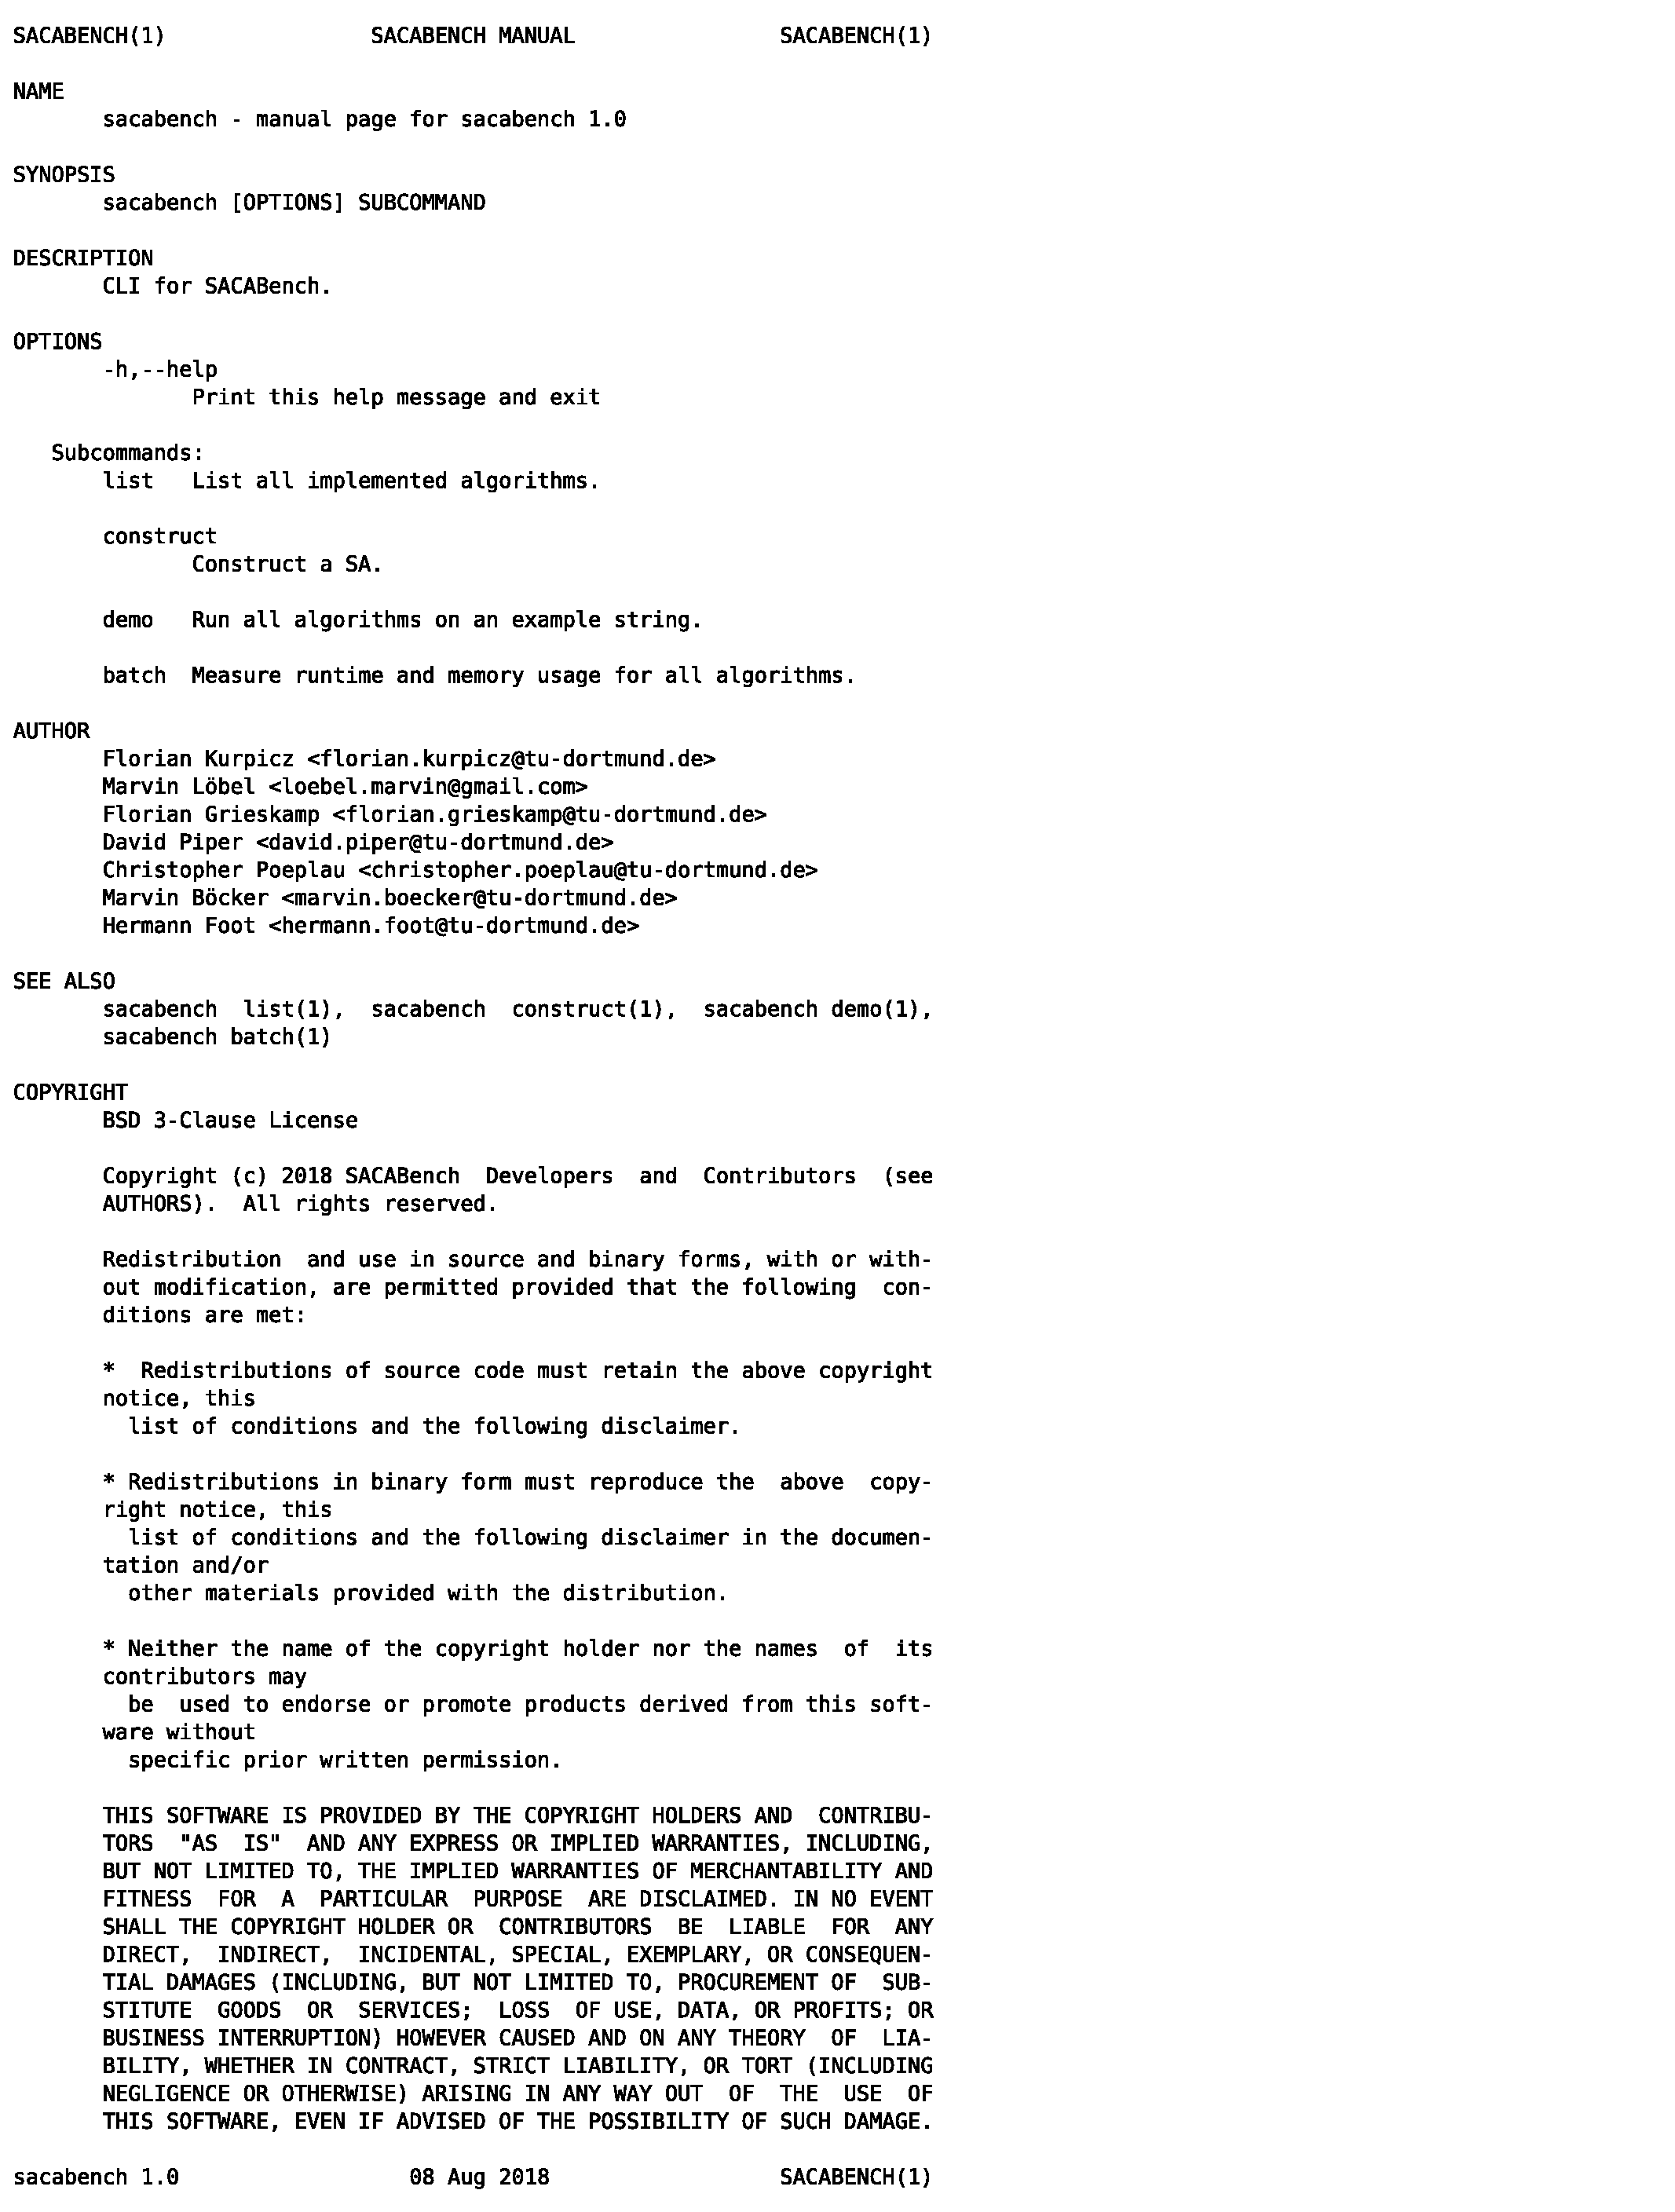
\includegraphics[page=1, viewport=0cm 32.8cm 20.5cm 47.5cm, clip, width=.5\textwidth]{{kapitel/3_framework/cli/sacabench/sacabench}.pdf}\\
    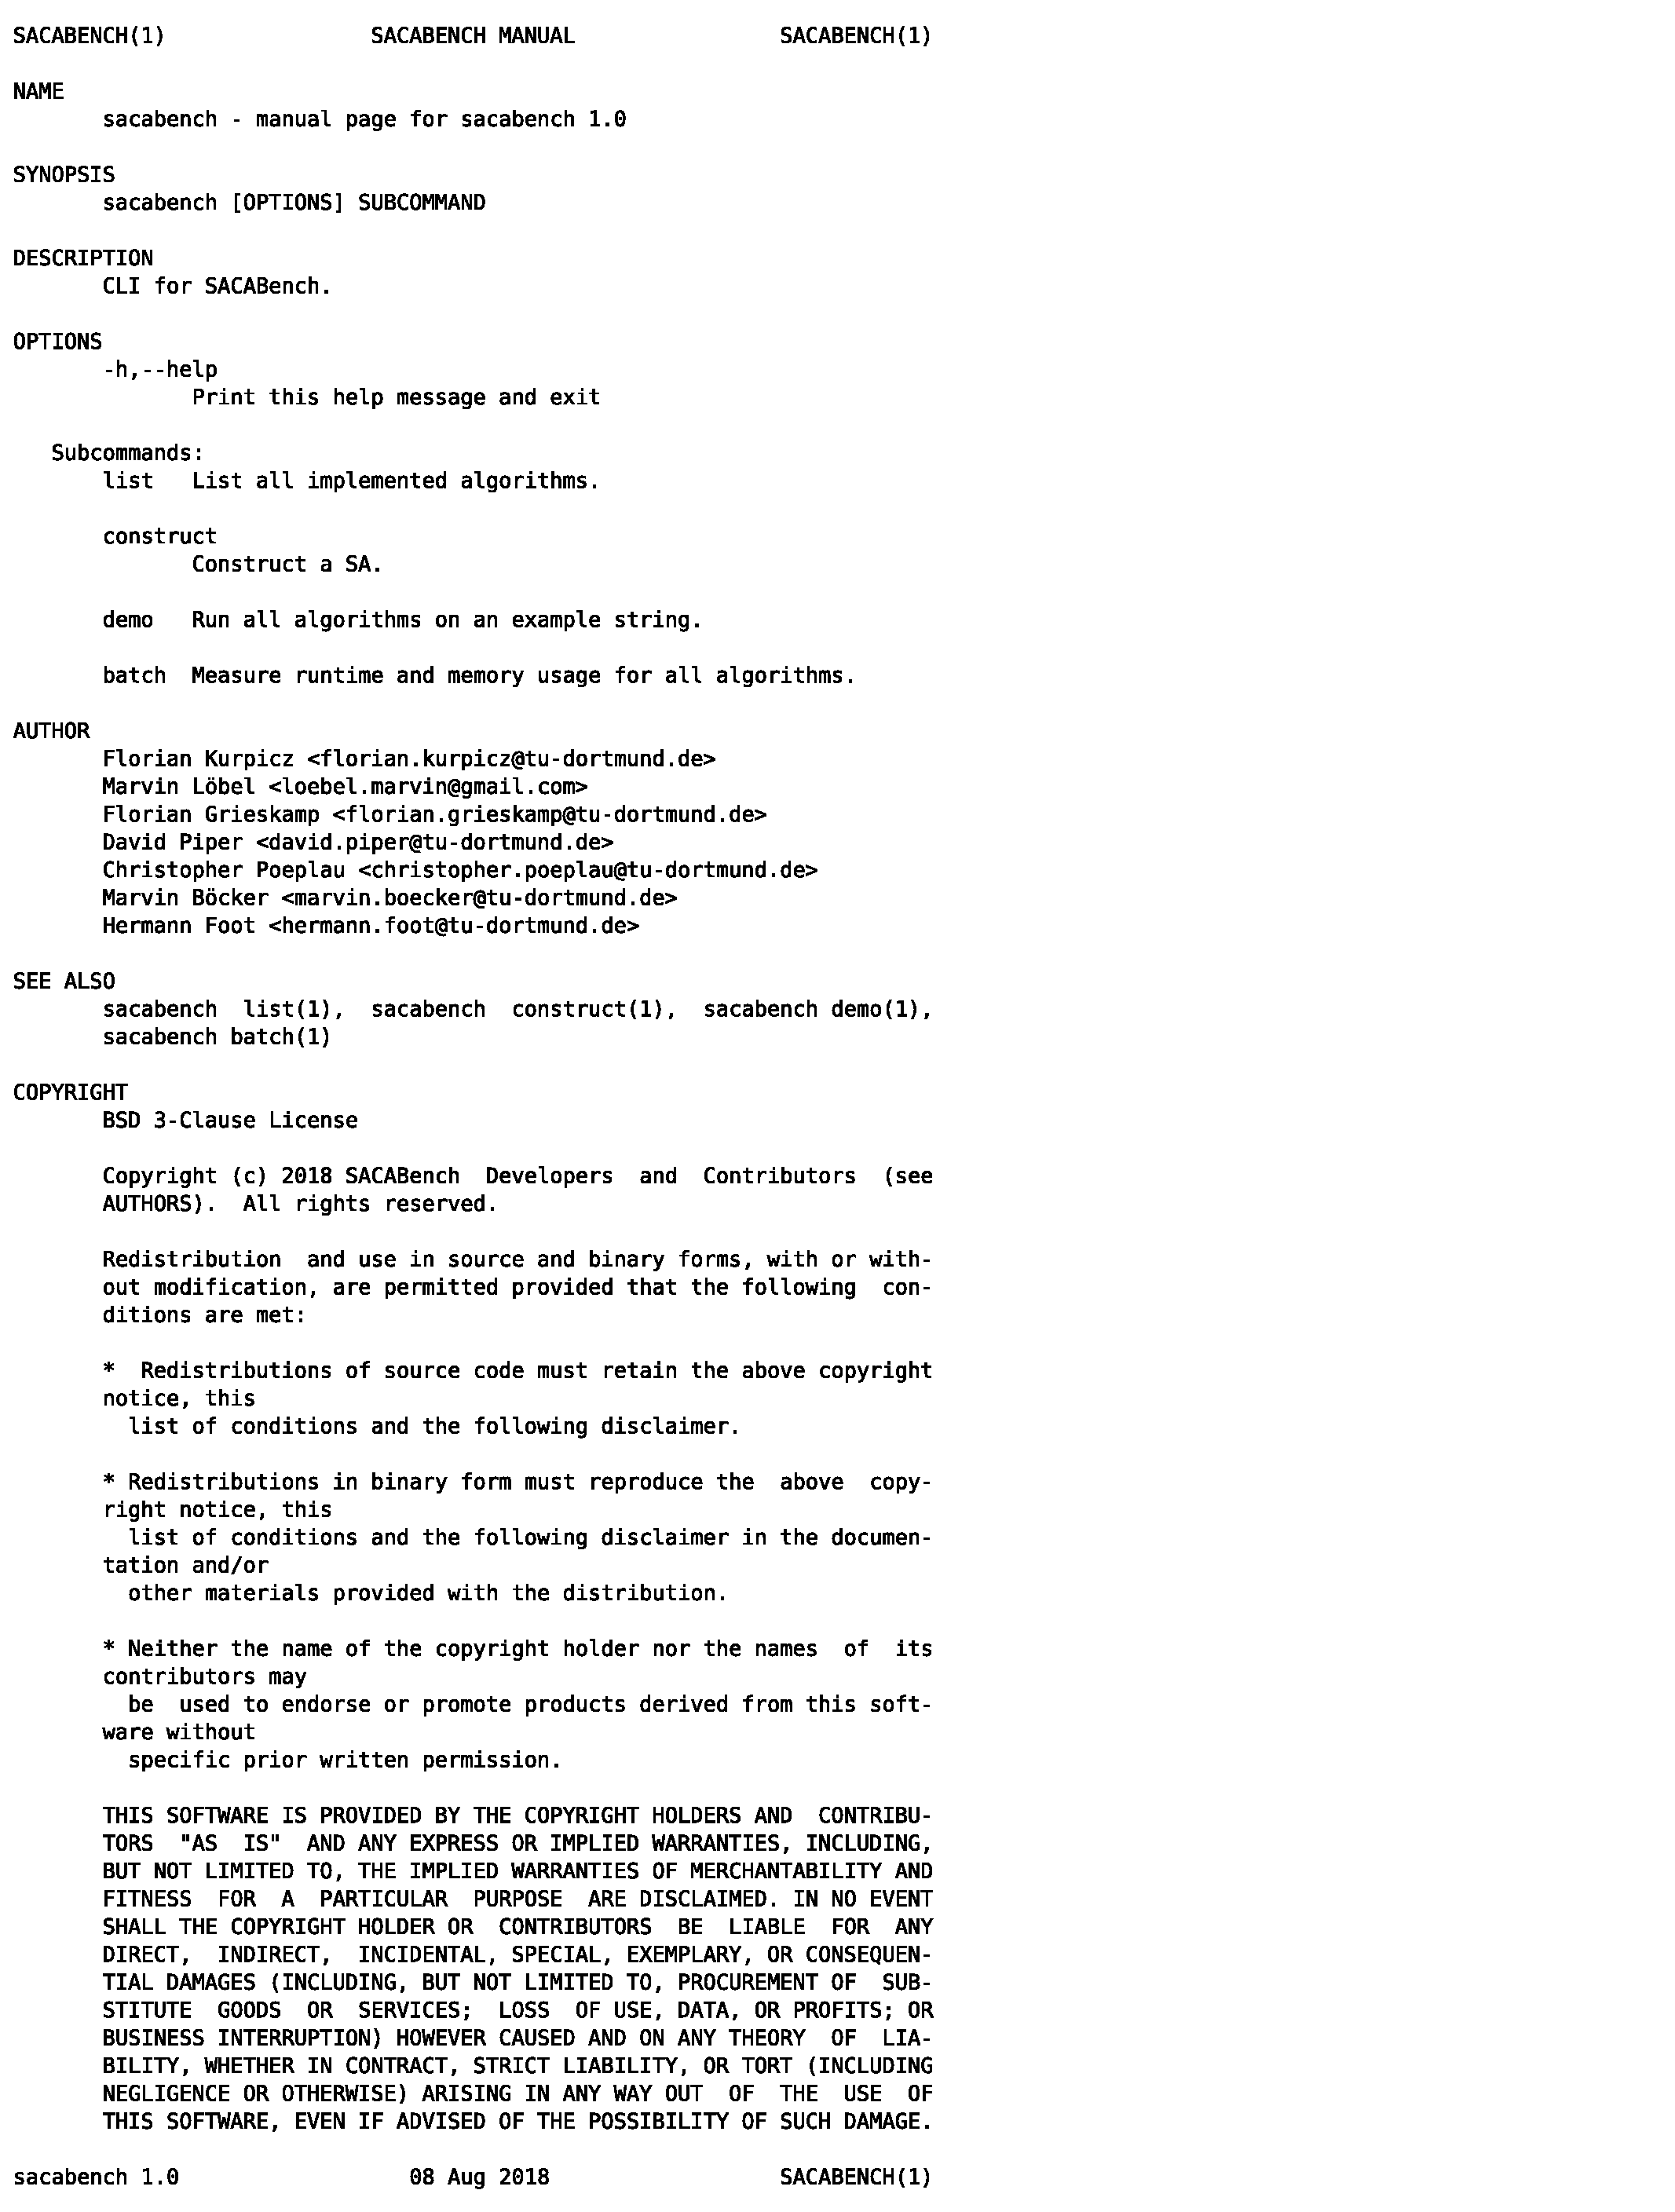
\includegraphics[page=1, viewport=0cm 25cm 20.5cm 27.3cm, clip, width=.5\textwidth]{{kapitel/3_framework/cli/sacabench/sacabench}.pdf}\\
    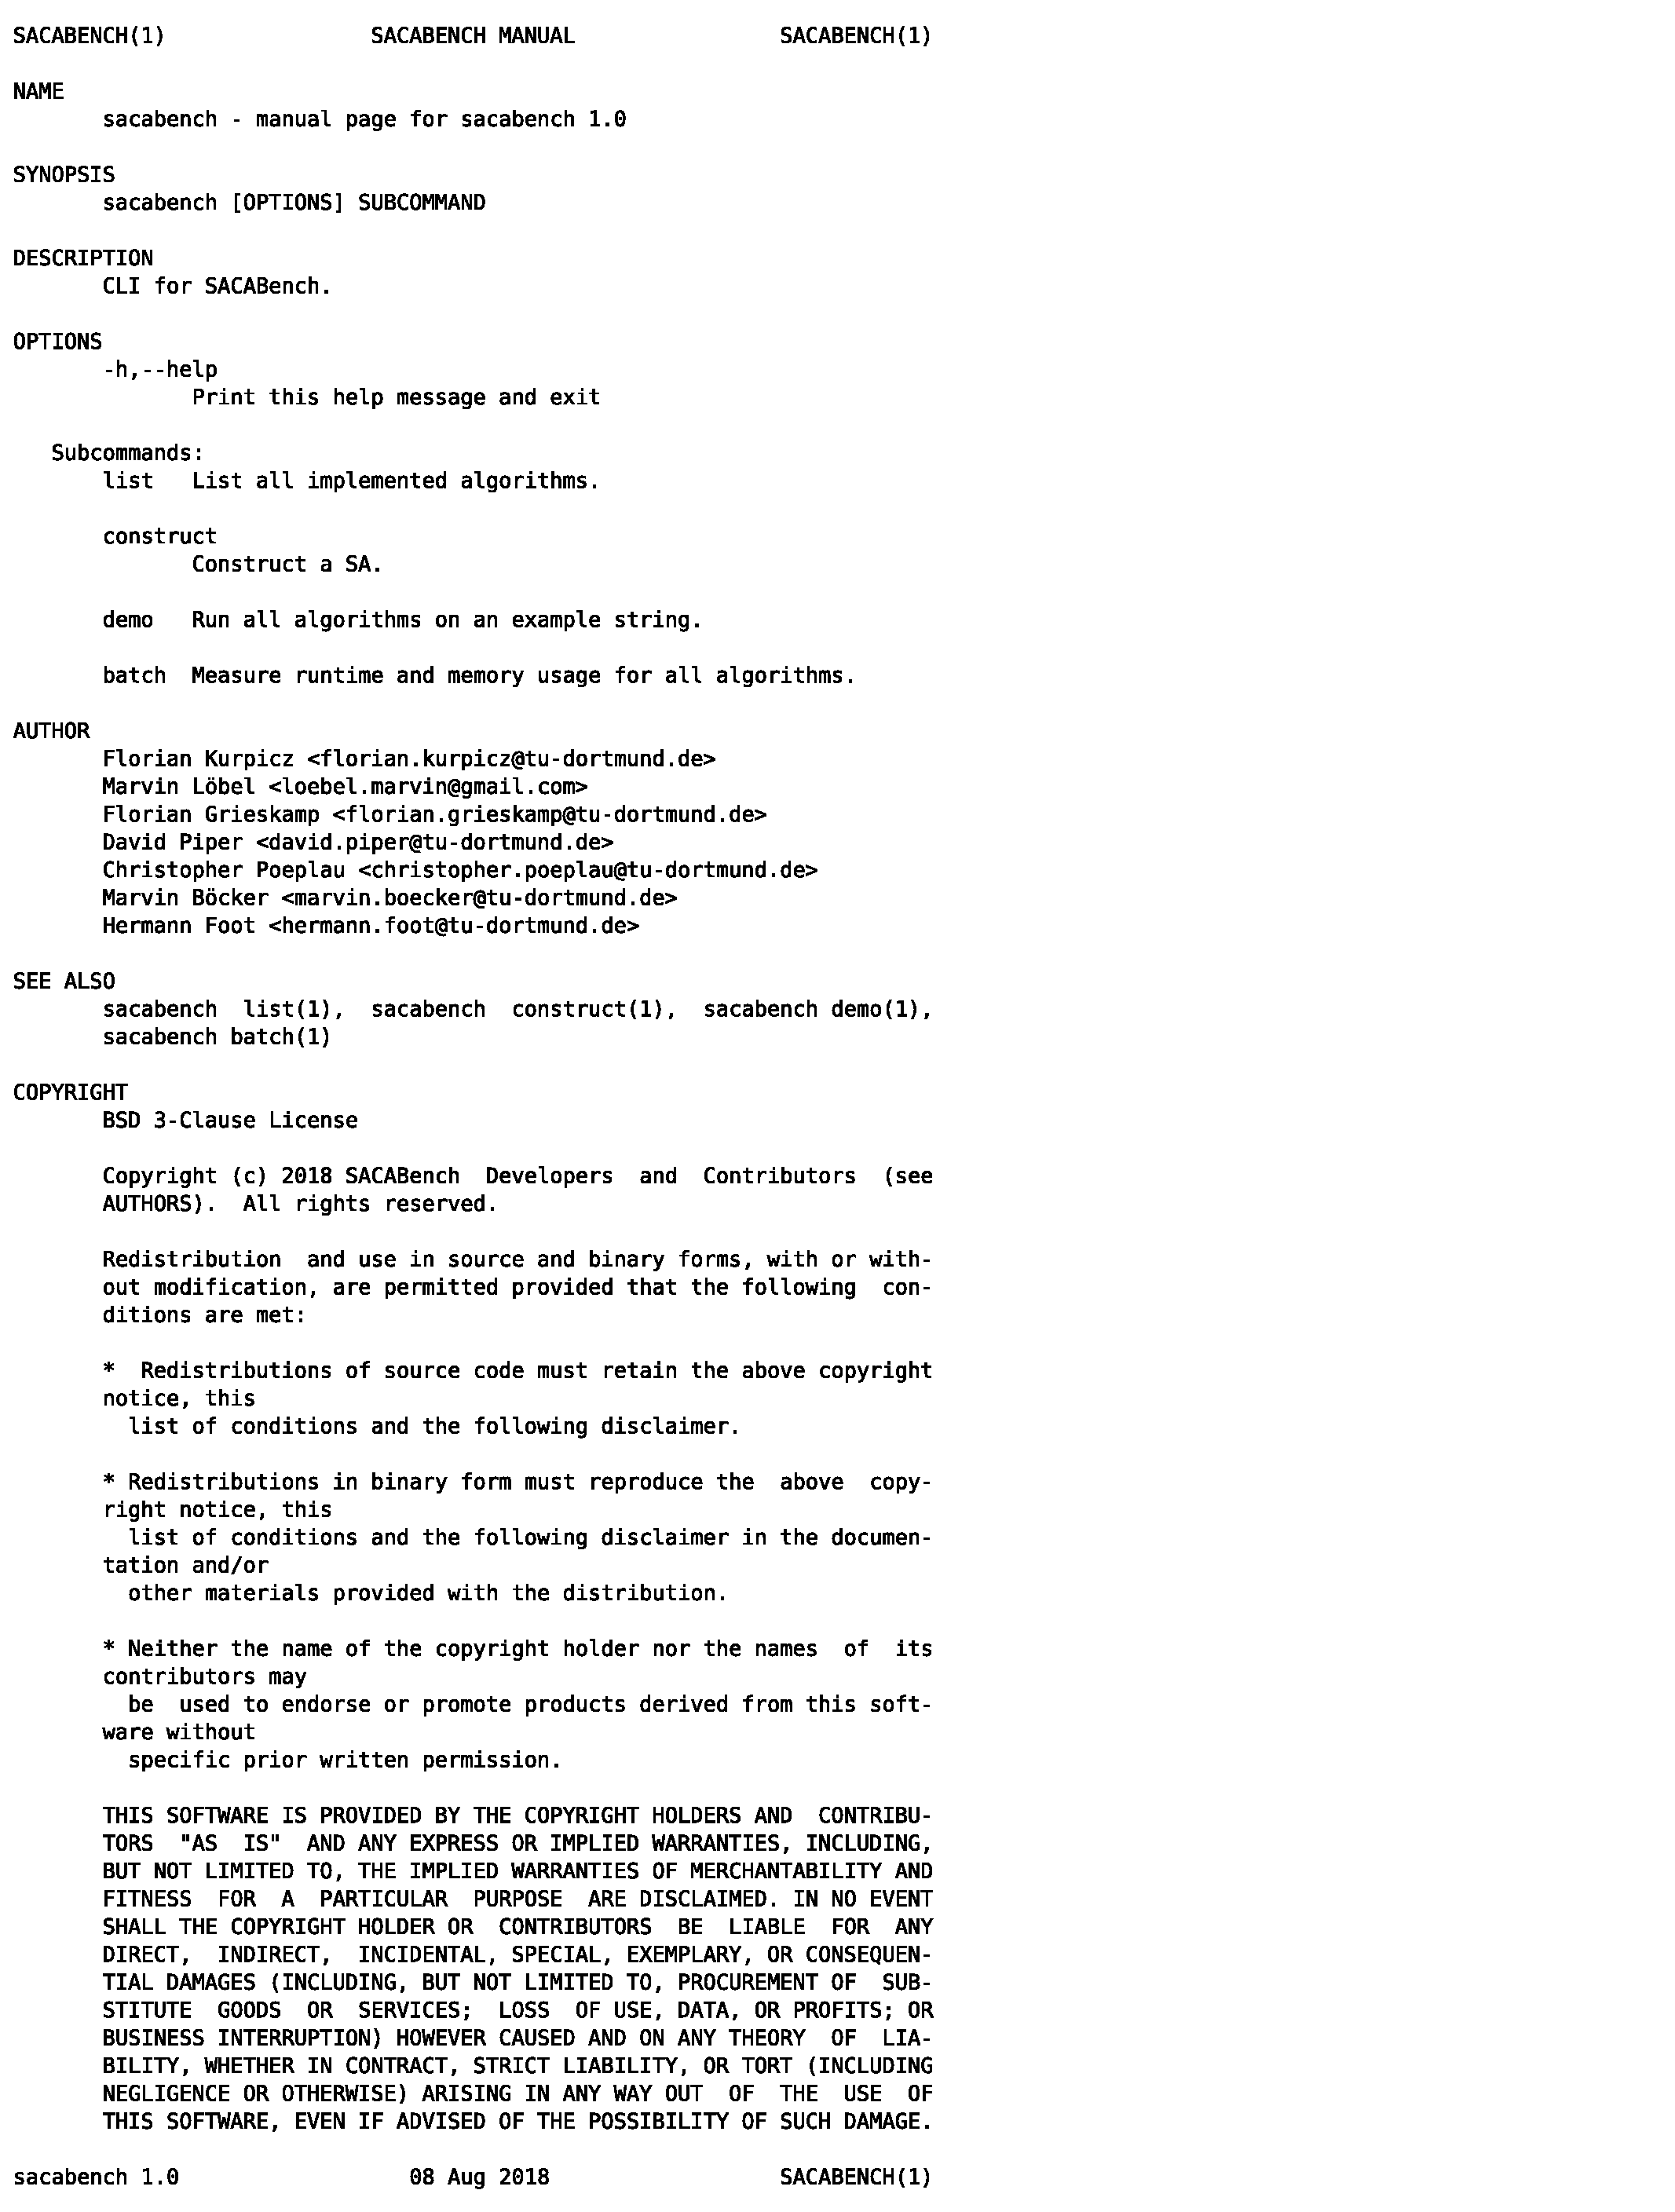
\includegraphics[page=1, viewport=0cm 0cm 20.5cm 1.5cm, clip, width=.5\textwidth]{{kapitel/3_framework/cli/sacabench/sacabench}.pdf}
    \caption{Gekürzte Ausgabe von \texttt{man sacabench}.}
    \label{manpage:sacabench}
\end{wrapfigure}
Das Hauptprogramm wird mit dem Befehl \texttt{sacabench} ausgeführt.
Für die einzelnen Funktionen stehen ent\-sprech\-ende Subcommands zur Verfügung.
Alle Komponenten beinhalten eine Hilfefunktion, die sich durch die Option \termfont{-h} bzw. \termfont{-{}-help} aufrufen lässt.
Die gleiche Hilfe wird außerdem ausgegeben, wenn das Programm mit ungültigen Parametern aufgerufen wird.
Für präzisere Erläuterungen der Aufrufe und Optionen stehen außerdem Man-Pages für alle Subcommands zur Verfügung.
Diese sind wie gewohnt über \termfont{man sacabench} bzw. \termfont{man sacabench [SUBCOMMAND]} aufzurufen und beinhalten neben der Beschreibung der Befehlssyntax und den Erläuterungen zur Verwendung der Optionen auch eine Liste der beteiligten Autoren, Verweise auf ähnliche Befehle und die Copyright-Bestimmungen.
Eine gekürzte Version der Man-Page für den Befehl \termfont{sacabench} ist in \cref{manpage:sacabench} zu sehen.
Alle im hier abgebildeten Man-Pages sind aus Gründen der Übersichtlichkeit um die Liste der Autoren und den Copyright-Verweis reduziert.\par
}

\subsection{sacabench list}
\label{framework:cli:sacabench-list}

Mit dem Befehl \texttt{sacabench list} können alle verfügbaren Algorithmen aufgelistet werden.
Nach dem Aufruf erscheint eine Liste aller im Rahmen der Projektgruppe implementierten Algorithmen, sowie deren Referenzimplementierungen. 
Letztere sind in der angegebenen Abkürzung durch \termfont{\_ref} markiert.\par
Über die Option \termfont{-{}-no-description} kann außerdem die Ausgabe der Kurz\-be\-schrei\-bungen unterdrückt werden, sodass nur noch eine Liste aller Kürzel erscheint. 
Die dort aufgelisteten Kürzel entsprechen den Bezeichnungen der Algorithmen, über die sie vom Framework referenziert werden.
Zusätzlich ermöglicht es die Option \termfont{-j} oder \termfont{-{}-json}, die Namen der Algorithmen als ein JSON Array auszugeben.\par

\subsection{sacabench demo}
\label{framework:cli:sacabench-demo}

{
\begin{wrapfigure}[9]{rR}[5mm]{.5\textwidth}
    \vspace{-1.5\baselineskip}
    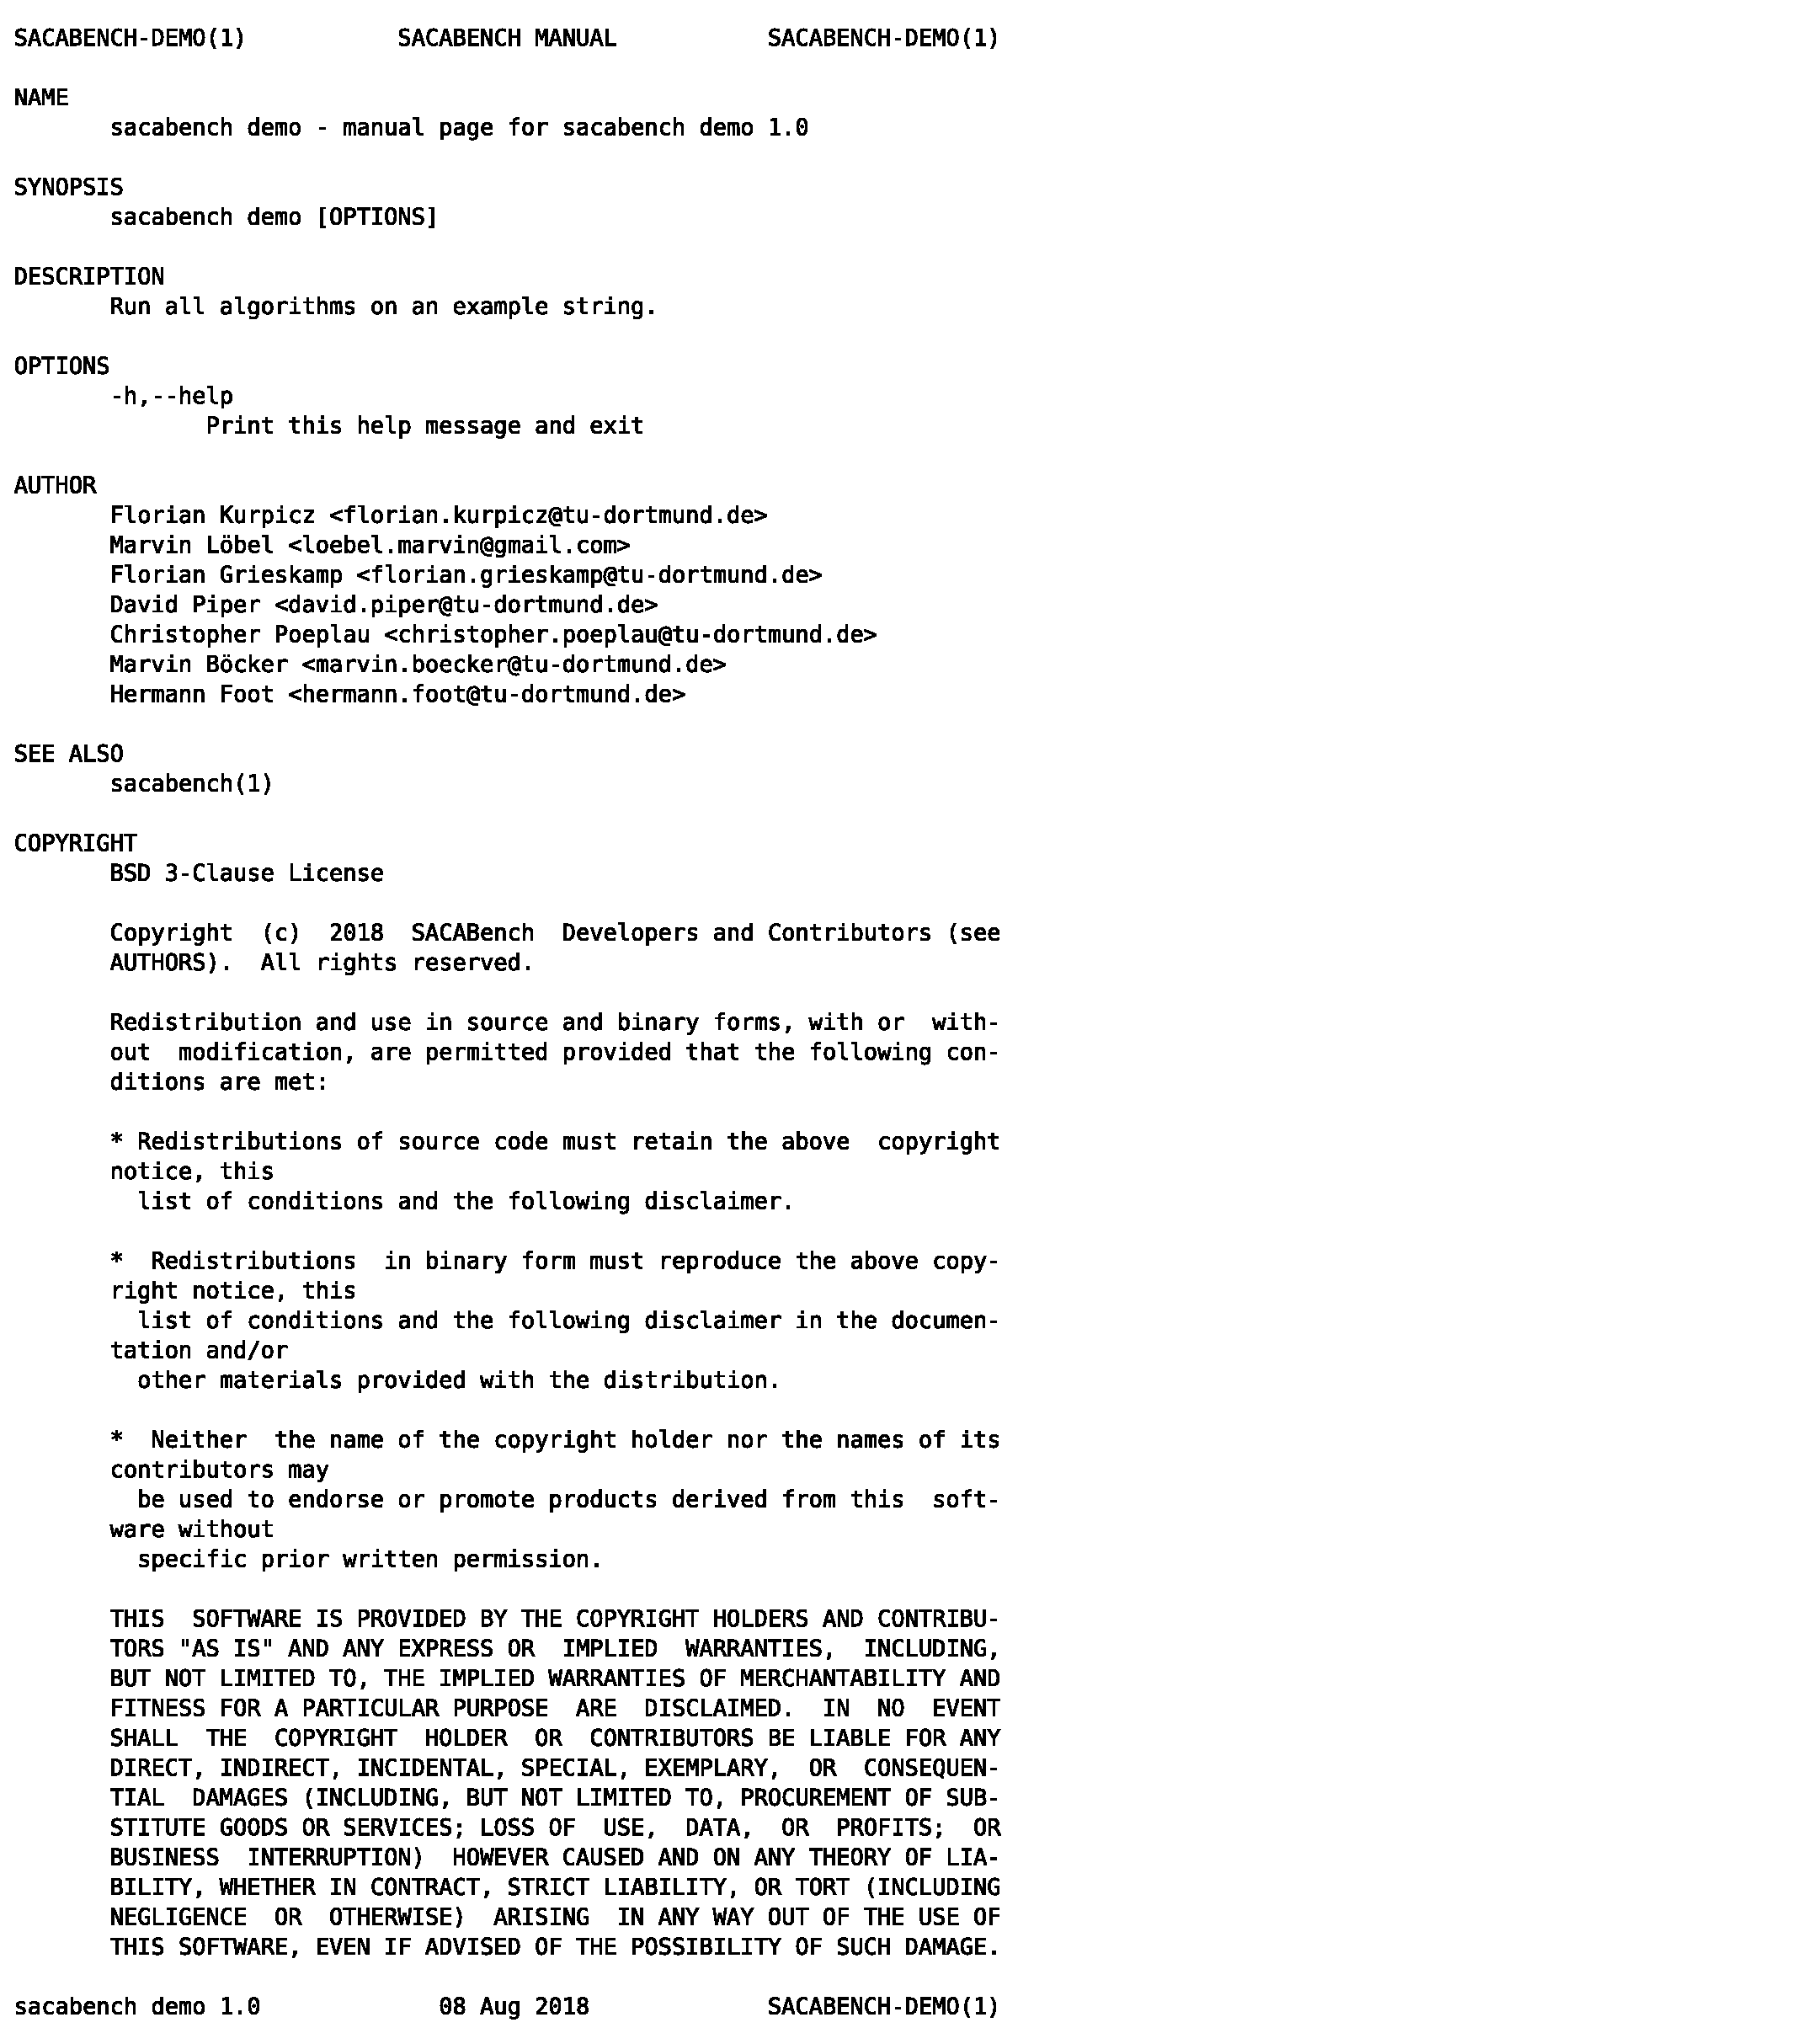
\includegraphics[page=1, viewport=0cm 32.8cm 20.5cm 41.0cm, clip, width=.5\textwidth]{{kapitel/3_framework/cli/sacabench-demo/sacabench-demo}.pdf}\\
    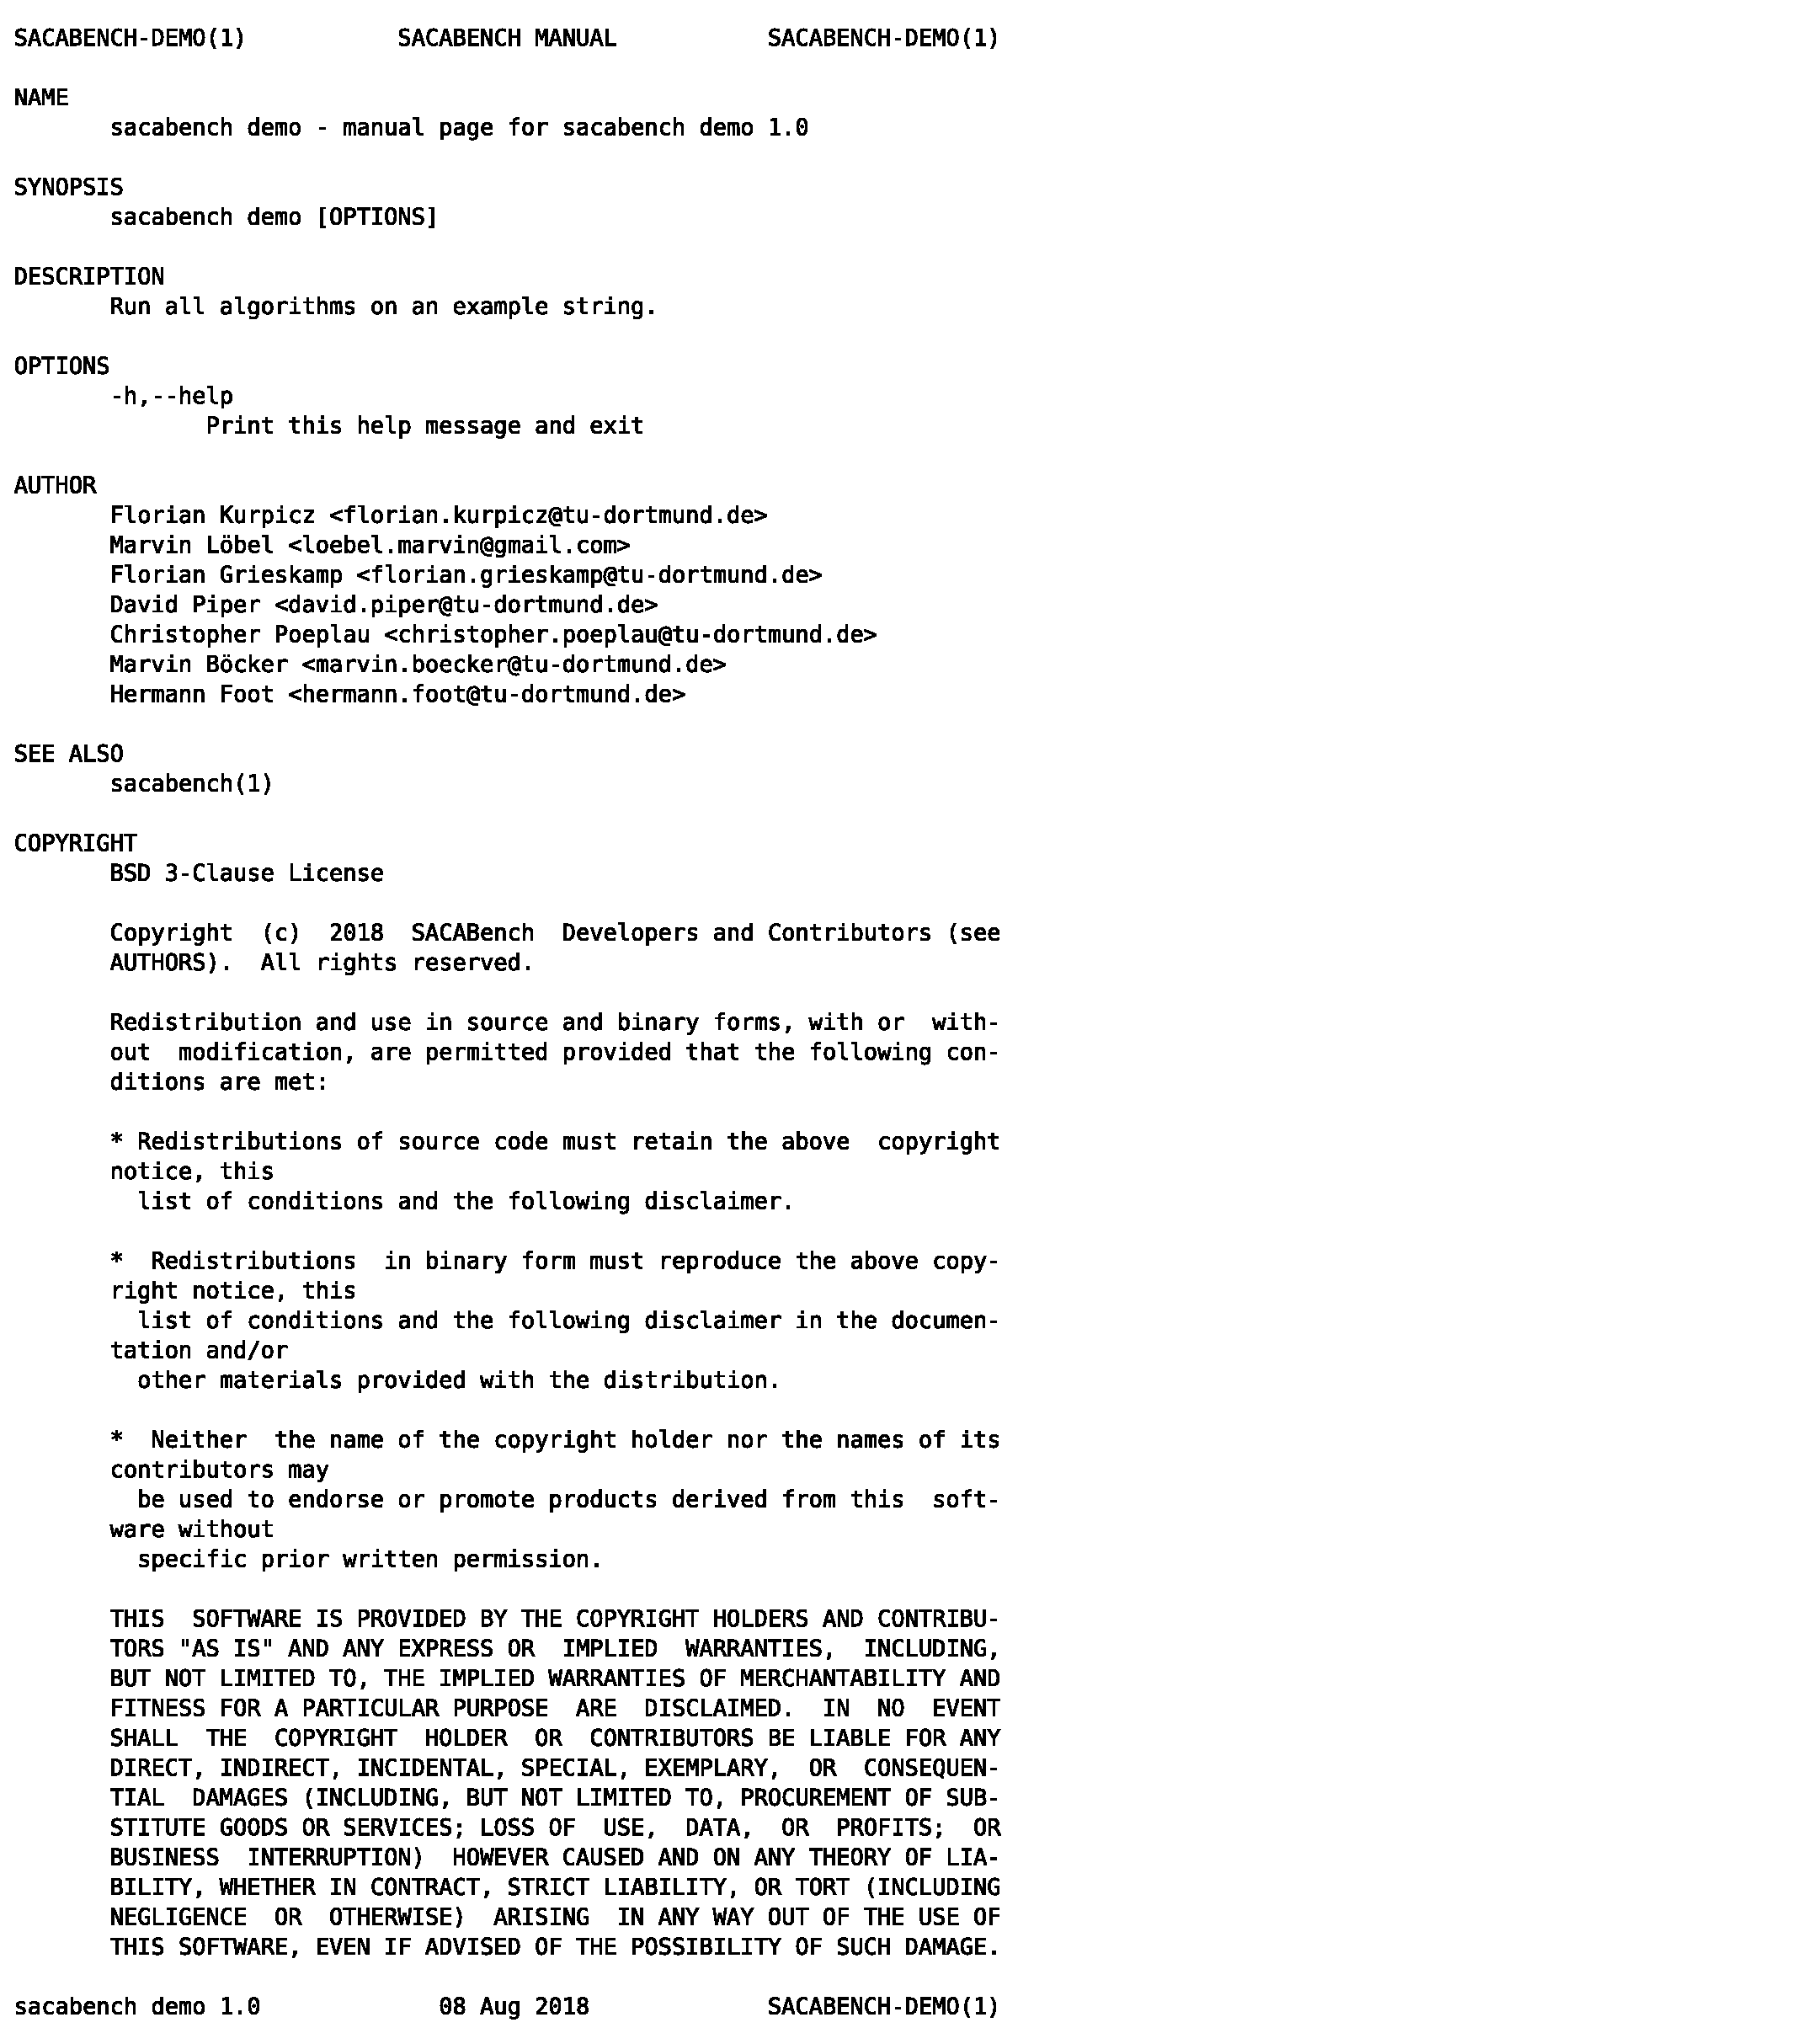
\includegraphics[page=1, viewport=0cm 25cm 20.5cm 26.3cm, clip, width=.5\textwidth]{{kapitel/3_framework/cli/sacabench-demo/sacabench-demo}.pdf}\\
    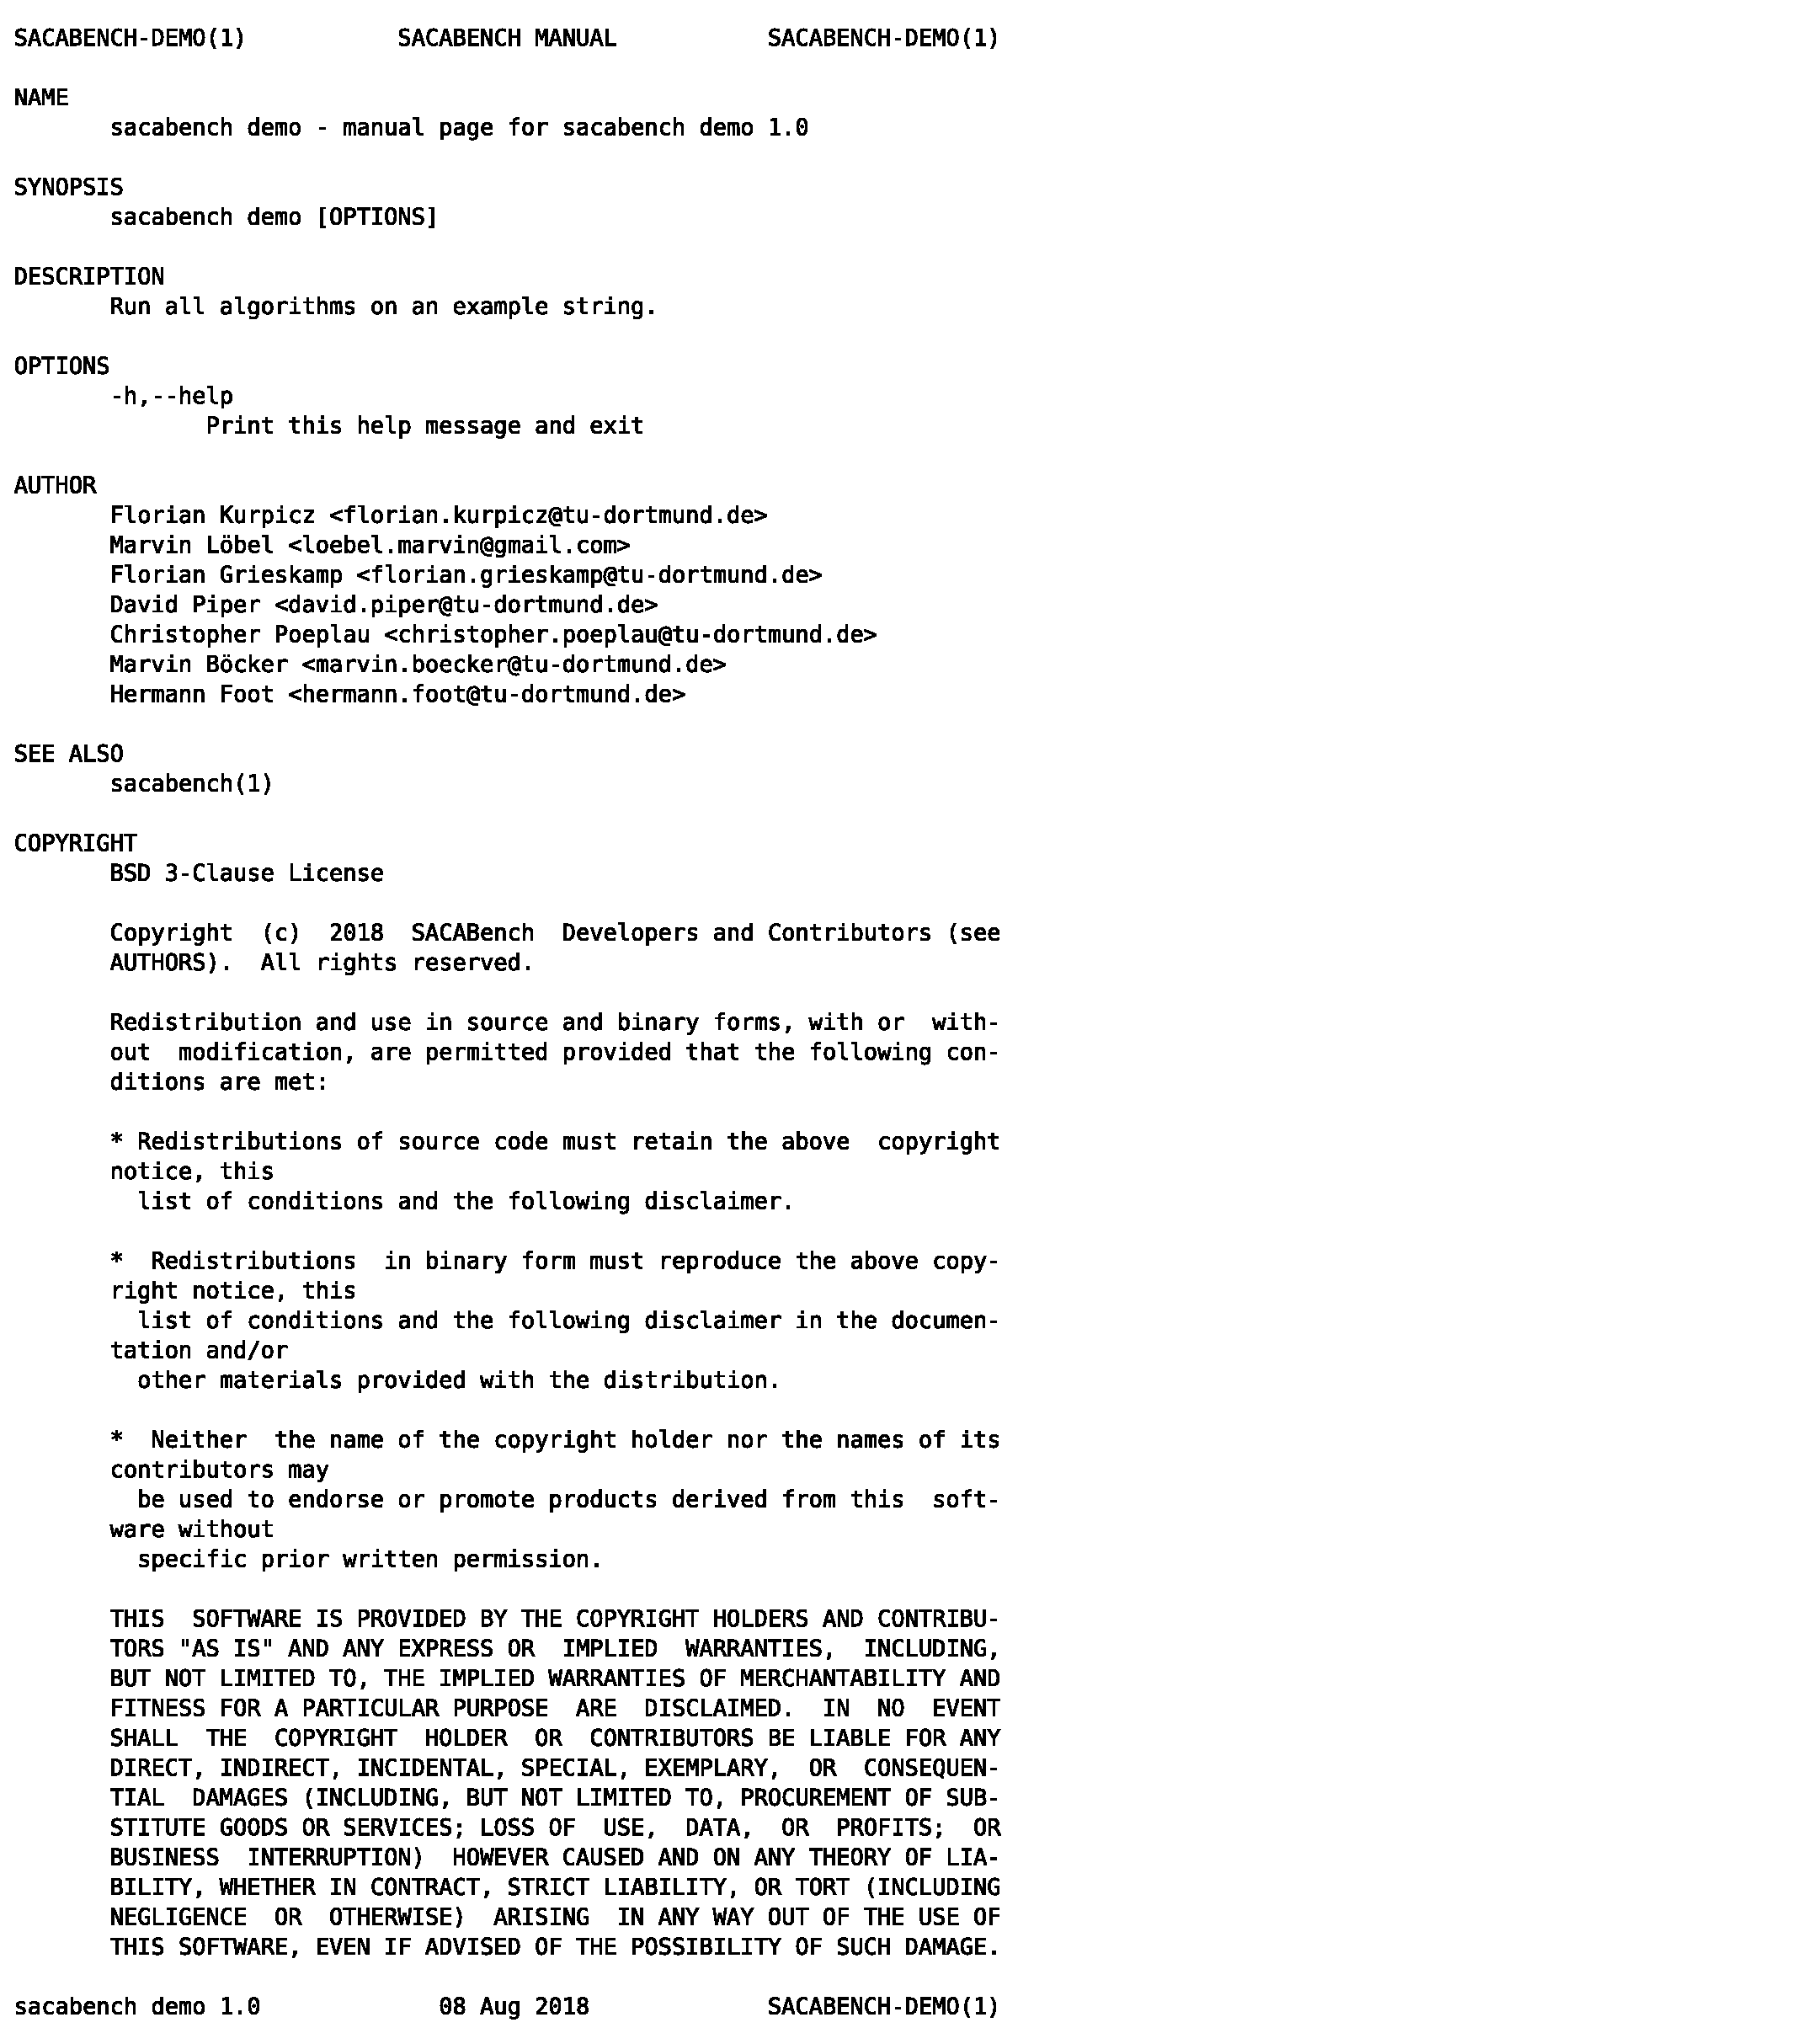
\includegraphics[page=1, viewport=0cm 0cm 20.5cm 1.5cm, clip, width=.5\textwidth]{{kapitel/3_framework/cli/sacabench-demo/sacabench-demo}.pdf}
    \caption{gekürzte Ausgabe von \texttt{man sacabench demo}}
    \label{manpage:sacabench-demo}
\end{wrapfigure}
Mit dem Befehl \texttt{sacabench demo} können alle Algorithmen auf einem kurzen Beispieltext (\glqq \termfont{hello world}\grqq) ausgeführt werden.\par
Diese Funktionalität erfüllt ausschließlich den Zweck, das Framework sowie die Algorithmen auf Lauffähigkeit auf dem verwendeten System zu testen. Auch hier ist eine Hilfeoption über \termfont{-h} bzw. \termfont{-{}-help} erreichbar.\par
}

\subsection{sacabench construct}
\label{framework:cli:sacabench-construct}

{
\begin{wrapfigure}[30]{R}[5mm]{.5\textwidth}
    \vspace{-1.5\baselineskip}
    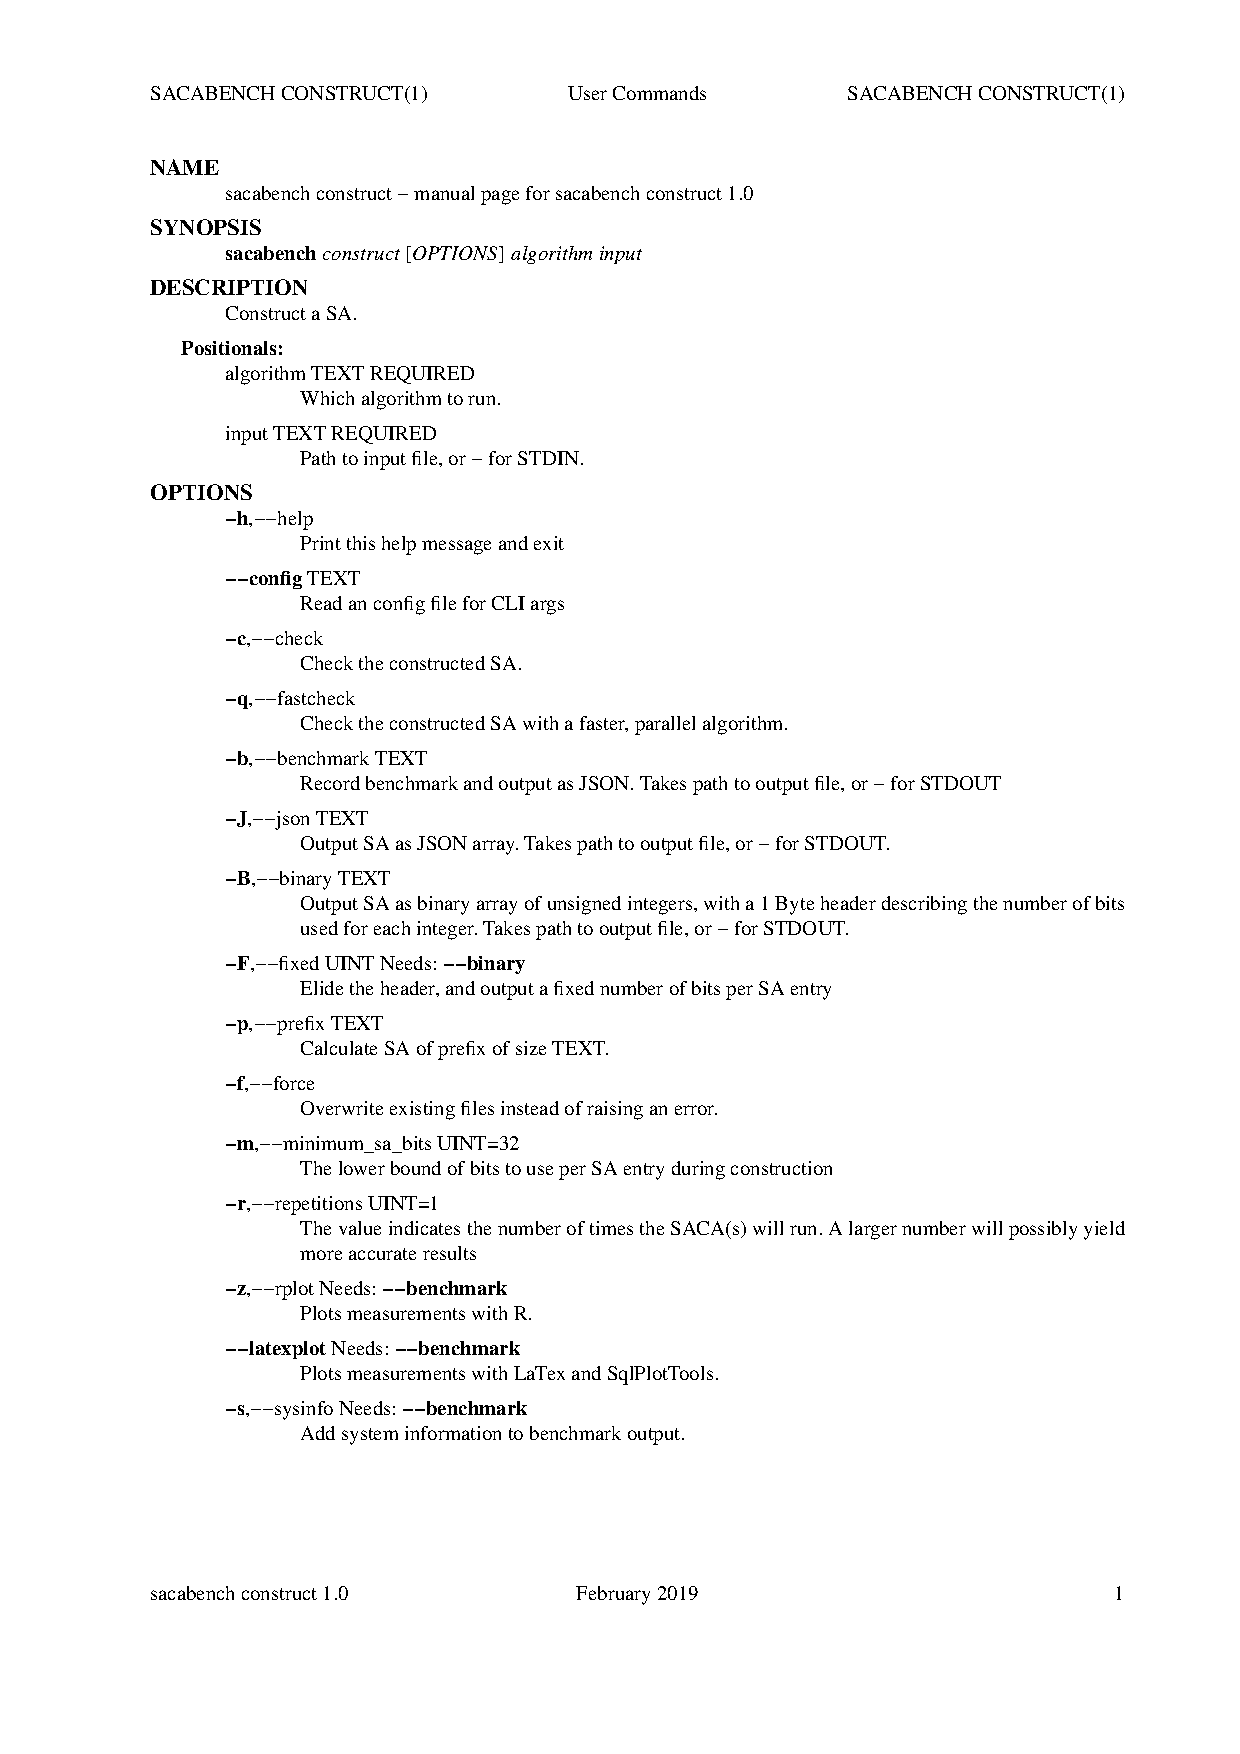
\includegraphics[page=1, viewport=0cm 32.8cm 20.5cm 68.5cm, clip, width=.5\textwidth]{{kapitel/3_framework/cli/sacabench-construct/sacabench-construct}.pdf}\\
    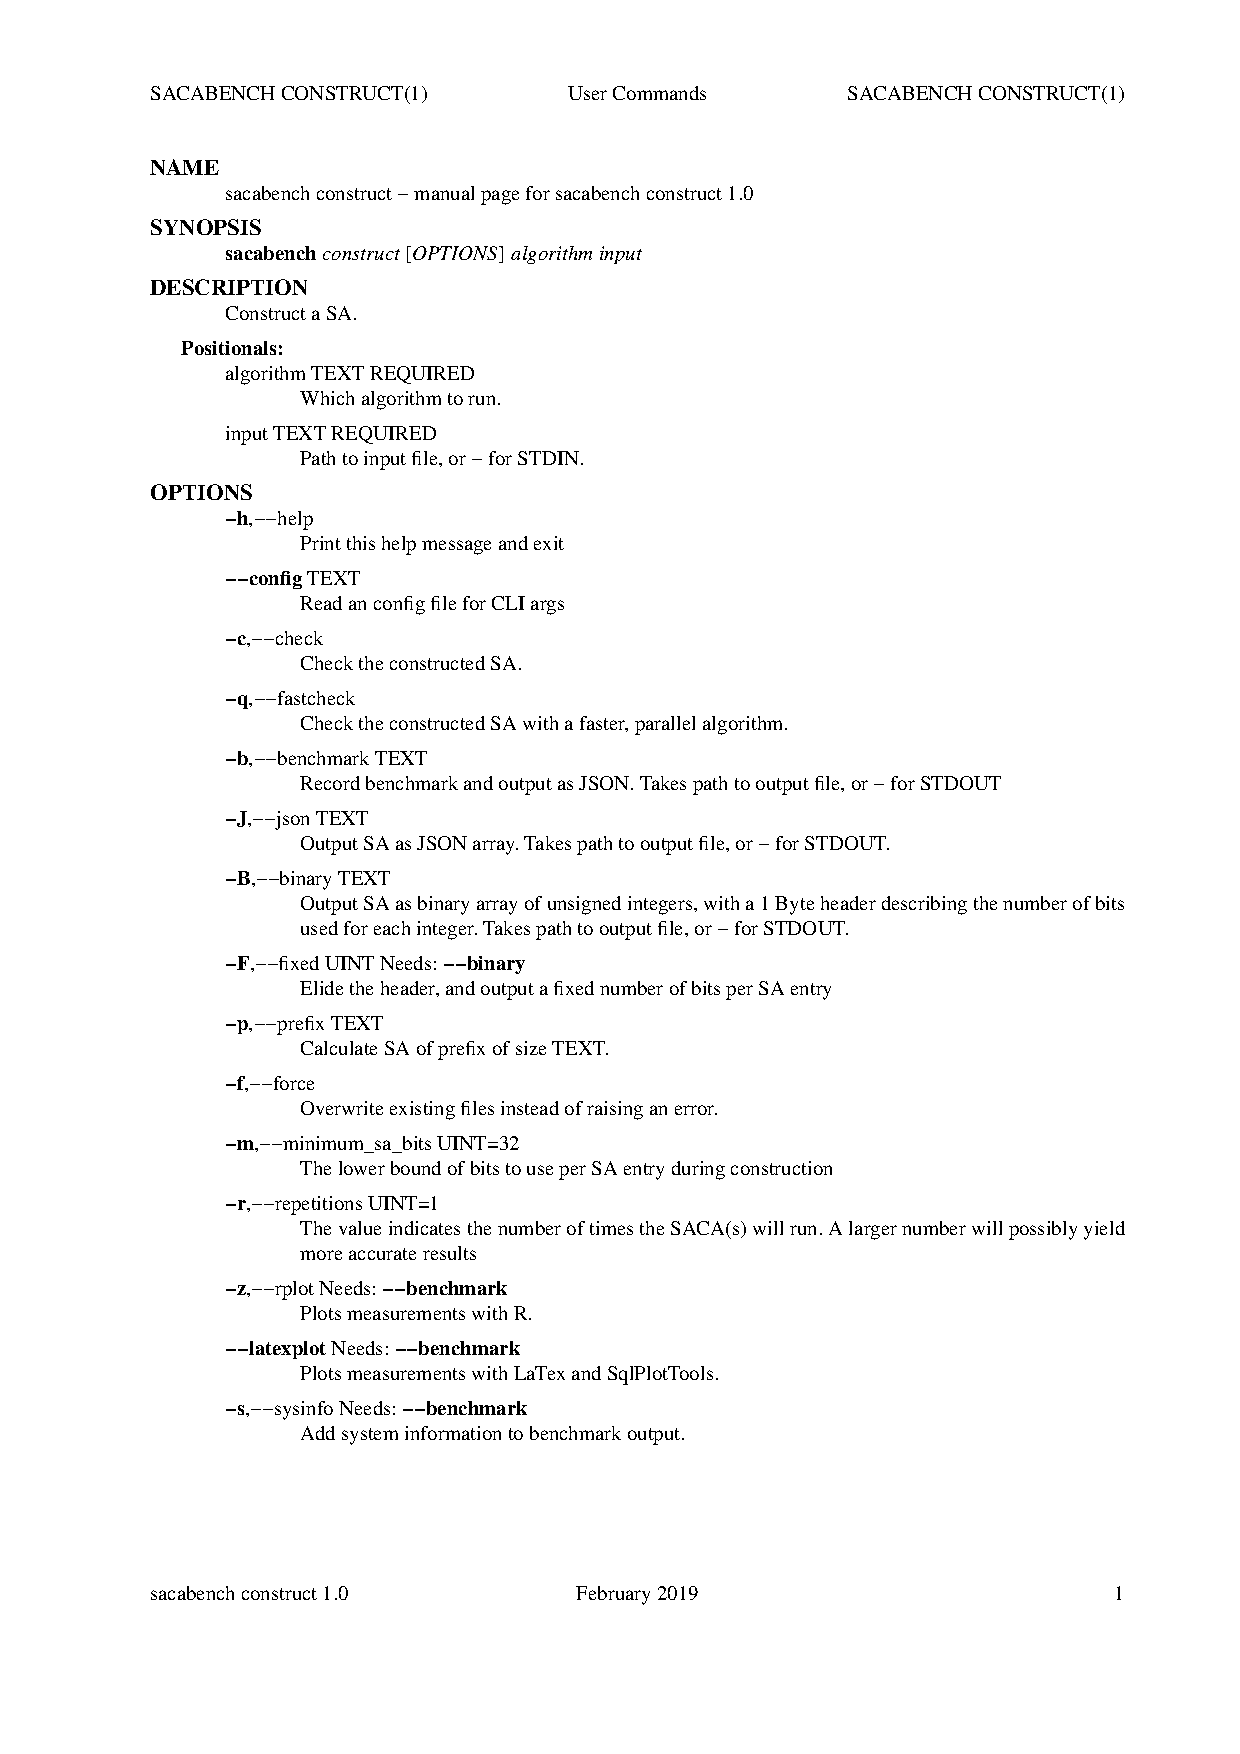
\includegraphics[page=1, viewport=0cm 25cm 20.5cm 26.3cm, clip, width=.5\textwidth]{{kapitel/3_framework/cli/sacabench-construct/sacabench-construct}.pdf}\\
    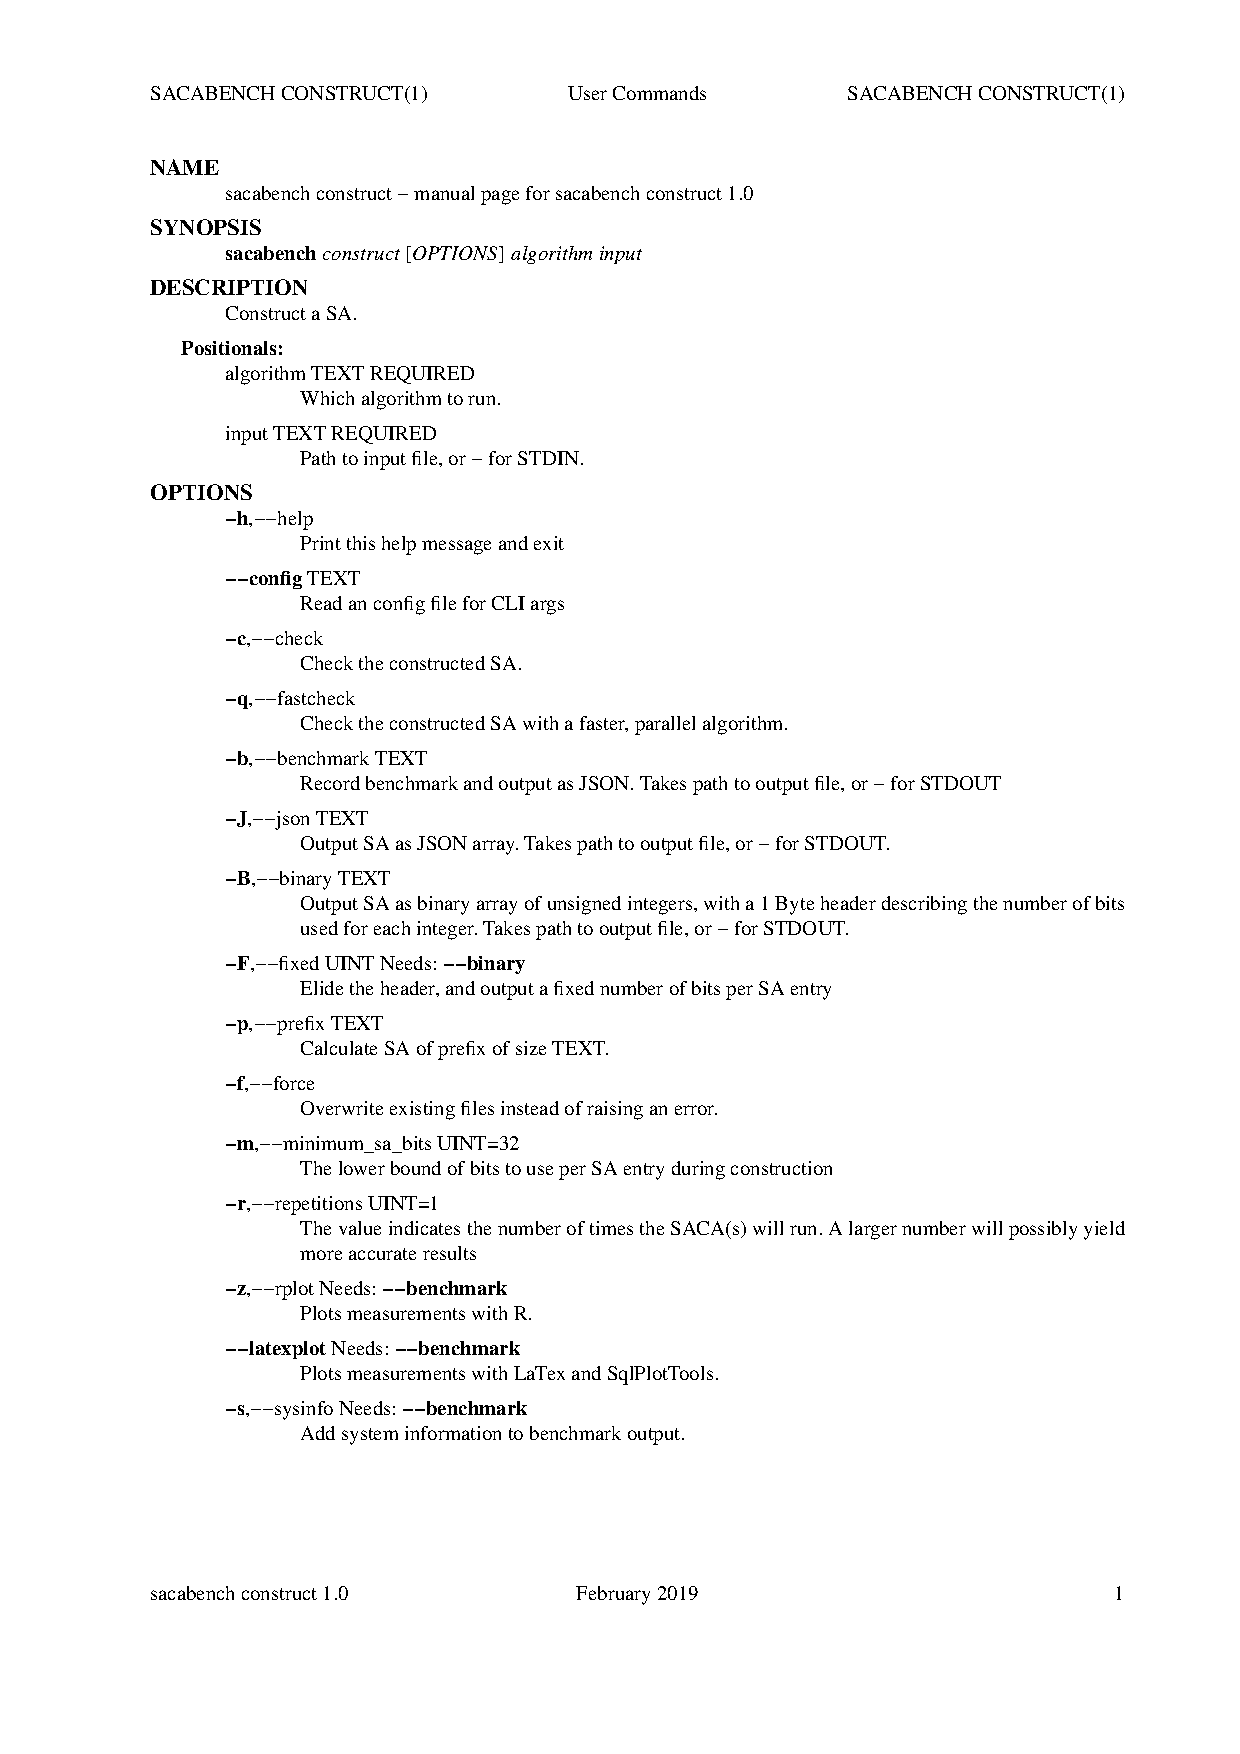
\includegraphics[page=1, viewport=0cm 0cm 20.5cm 1.5cm, clip, width=.5\textwidth]{{kapitel/3_framework/cli/sacabench-construct/sacabench-construct}.pdf}
    \caption{gekürzte Ausgabe von \texttt{man sacabench construct}}
    \label{manpage:sacabench-construct}
\end{wrapfigure}

Mit dem Befehl \texttt{sacabench construct} kann ein ausgewählter Algorithmus ausgeführt werden. 
\par
Der auszuf{\"u}hrende Algorithmus wird dabei durch sein K{\"u}rzel bestimmt, wie es bei \termfont{sacabench list} angegeben ist. 
Gefolgt wird der Name des Algorithmus durch den Text, auf den er angewendet werden soll. 
Hierf{\"u}r kann ein Pfad zu einer Textdatei oder alternativ \termfont{-} f{\"u}r STDIN angegeben werden. 
\par
Zus{\"a}tzlich kann eine ganze Reihe von Optionen angegeben werden. 
Wie auch bei anderen Subcommands zeigen \termfont{-h} und \termfont{-{}-help} die Hilfe an. 
Die Option \termfont{-c} bzw. \termfont{-{}-check} wendet zus{\"a}tzlich zu dem ausgew{\"a}hlten Algorithmus einen weiteren SACA auf die Eingabe an und {\"u}berpr{\"u}ft, ob die beiden Ergebnisse gleich sind. 
Ist dies nicht der Fall, wird eine Fehlermeldung angezeigt. 
Eine Alternative hierzu ist die Option \termfont{-q} oder \termfont{-{}-quick}, welche auch die Korrektheit überprüft, jedoch einen parallelen Algorithmus verwendet. 
Wird die Option \termfont{-b} oder \termfont{-{}-benchmark} gefolgt von einem Pfad angegeben, wird an diesem Pfad eine JSON-Datei mit den gemessenen Zeiten und Speicherverbrauch angelegt. 
Existiert an dem angegebenen Pfad bereits eine Datei, kann diese mit der Option \termfont{-f} bzw. \termfont{-{}-force} {\"u}berschrieben und durch die neue Messung ersetzt werden. 
Der Inhalt dieser Datei ist die Grundlage f{\"u}r die durch ein R-Skript erstellten Diagramme, welche mit \termfont{-z} oder \termfont{-{}-rplot} bei der Ausf{\"u}hrung des Algorithmus generiert werden. 
Als Alternative hierzu können durch die Option \termfont{-{}-latexplot} auch Plots durch SqlPlotTools und Latex generiert werden.
Weitere Informationen hierzu sind in Kapitel \ref{framework:bechmark:sqlplottools} enthalten.
Um bei den Messungen ein besseres Ergebnis zu erhalten, kann mit der Option \termfont{-r} bzw. \termfont{-{}-repetitions} eine Anzahl an Durchf{\"u}hrungen festgelegt werden. 
Hierdurch wird die Genauigkeit der Messung erh{\"o}ht, indem das Arithmetische Mittel gebildet wird.
Weiterhin kann dem Befehl \termfont{-p} oder \termfont{-{}-prefix} hinzugef{\"u}gt werden. 
Hierbei kann die Anzahl an f{\"u}hrenden Bytes angegeben werden, die von der Eingabe verarbeitet werden sollen.
Um gr{\"o}{\ss}ere Werte leichter angeben zu k{\"o}nnen, sind die Abk{\"u}rzenden Schreibweisen K und M erlaubt, welche f{\"u}r Kilobyte bzw. Megabyte stehen.
Dies sorgt daf{\"u}r, dass von der {\"u}bergebenen Textdatei nur so viele Bytes verarbeitet werden, wie durch diese Option angegeben werden. 
Die Option \termfont{-B} oder \termfont{-{}-binary} veranlasst das Framework zur Ausgabe in bin{\"a}rer Form.
Anschlie{\ss}end werden die Eintr{\"a}ge des Ergebnisses als Bin{\"a}rzahlen mit bis zu 8 Stellen ausgegeben. 
Die erste Zahl der Ausgabe gibt die genaue Anzahl der Stellen an.
Ist eine feste Anzahl an Bits gew{\"u}nscht, kann diese mit der Option \termfont{-F} bzw. \termfont{-{}-fixed} angegeben werden.
Alternativ kann das Framework das Suffixarray als JSON-Array ausgeben. 
Dies ist mit der Option \termfont{-J} oder \termfont{-{}-json} möglich.
Die nächste Option, welche dem Subcommand \texttt{sacabench construct} {\"u}bergeben werden kann, ist \termfont{-m} oder \termfont{-{}-minimum\_sa\_bits} gefolgt von einem UINT Wert. 
Dieser Parameter bestimmt die Anzahl der Bits, die f{\"u}r die Datenstrukturen w{\"a}hrend der Berechnung genutzt werden.
Anstatt diese Optionen einzeln anzugeben, kann auch eine Konfigurationsdatei eingelesen werden, welche Werte für die zu benutzenden Optionen angibt.
Diese Datei ist im ini-Format und anstelle der Optionen wird die Option \termfont{-{}-config} gefolgt zu dem Pfad zu der Konfigurations-Datei beim Aufruf dieses Befehls angegeben.
Ein Beispiel für solch eine Konfigurations-Datei ist in Abbildung \ref{sacabench-construct:config} zu sehen.
Soll das Tool beispielsweise für den SACA \texttt{BPR} mit der angezeigten Konfigurationsdatei aufgerufen werden, sieht der entsprechende Befehl folgendermaßen aus:

\termfont{sacabench/sacabench construct --config /pfad/zur/config BPR \linebreak /pfad/zum/input/text}

Die gezeigte Konfigurations-Datei ist gleichbedeutentd zum Aufruf mit den Optionen \termfont{-c}, \termfont{-b}, \termfont{-f}, \termfont{-p 1K}, \termfont{-r 2}, \termfont{--rplot} und \termfont{--latexplot}.
Sollen die Optionen einzeln übergeben werden, ist dies mit diesem Aufruf möglich:

\termfont{sacabench/sacabench construct -c -b /ziel/pfad/zur/ergebnis.json -f -p 1K -r 2 --rplot --latexplot BPR /pfad/zum/input/text}
\par
}
\begin{figure}[!h]
\begin{minted}
[
frame=lines,
framesep=2mm,
baselinestretch=1.2,
fontsize=\footnotesize,
linenos,
numbersep=-4mm,
breaklines,
escapeinside=@@,
frame=single,
framesep=14pt
]
{text}
check = true
benchmark = /ziel/pfad/zur/ergebnis.json
force = true
prefix = 1K
repetitions = 2
rplot = true
latexplot = true
\end{minted}
\caption[Beispiel für eine Konfigurations-Datei für den Befehl \texttt{sacabench construct}]{Beispiel für eine Konfigurations-Datei für den Befehl \texttt{sacabench construct}}
\label{sacabench-construct:config}
\end{figure}

\subsection{sacabench batch}
\label{framework:cli:sacabench-batch}

{
    \begin{wrapfigure}[25]{r}[5mm]{.5\textwidth}
    \vspace{-1.5\baselineskip}
    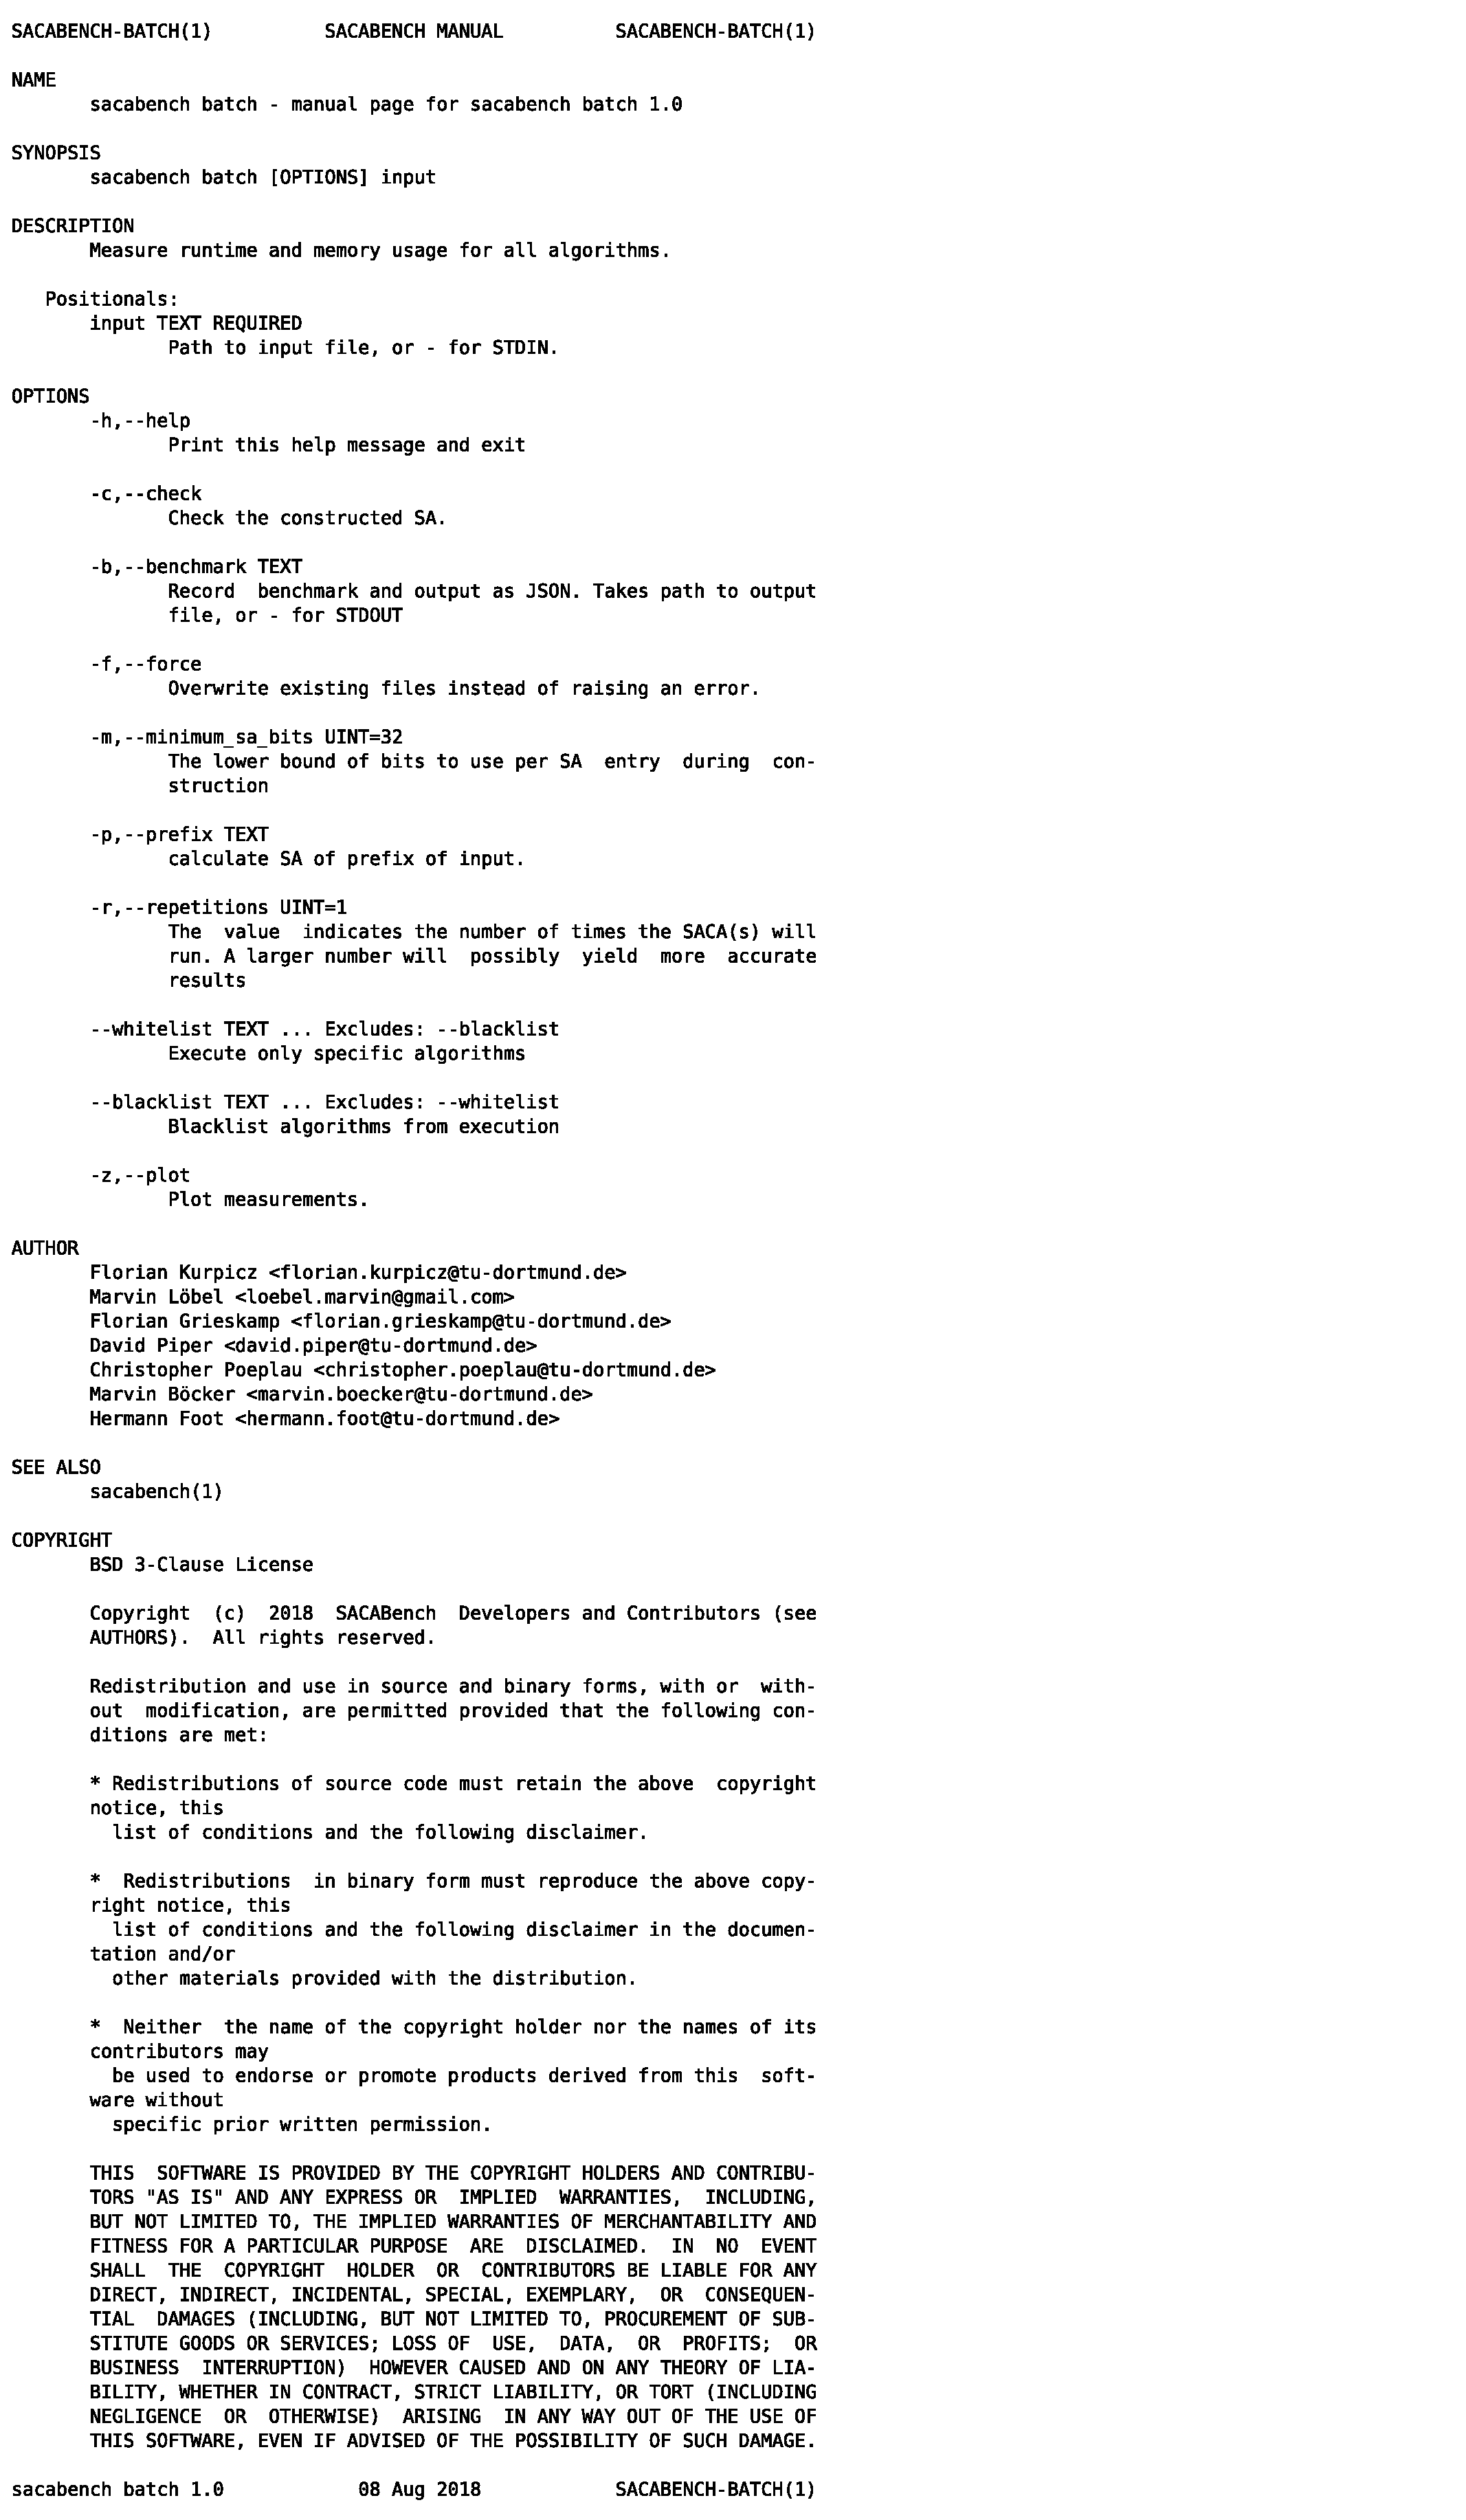
\includegraphics[page=1, viewport=0cm 32.8cm 20.5cm 62.0cm, clip, width=.5\textwidth]{{kapitel/3_framework/cli/sacabench-batch/sacabench-batch}.pdf}\\
    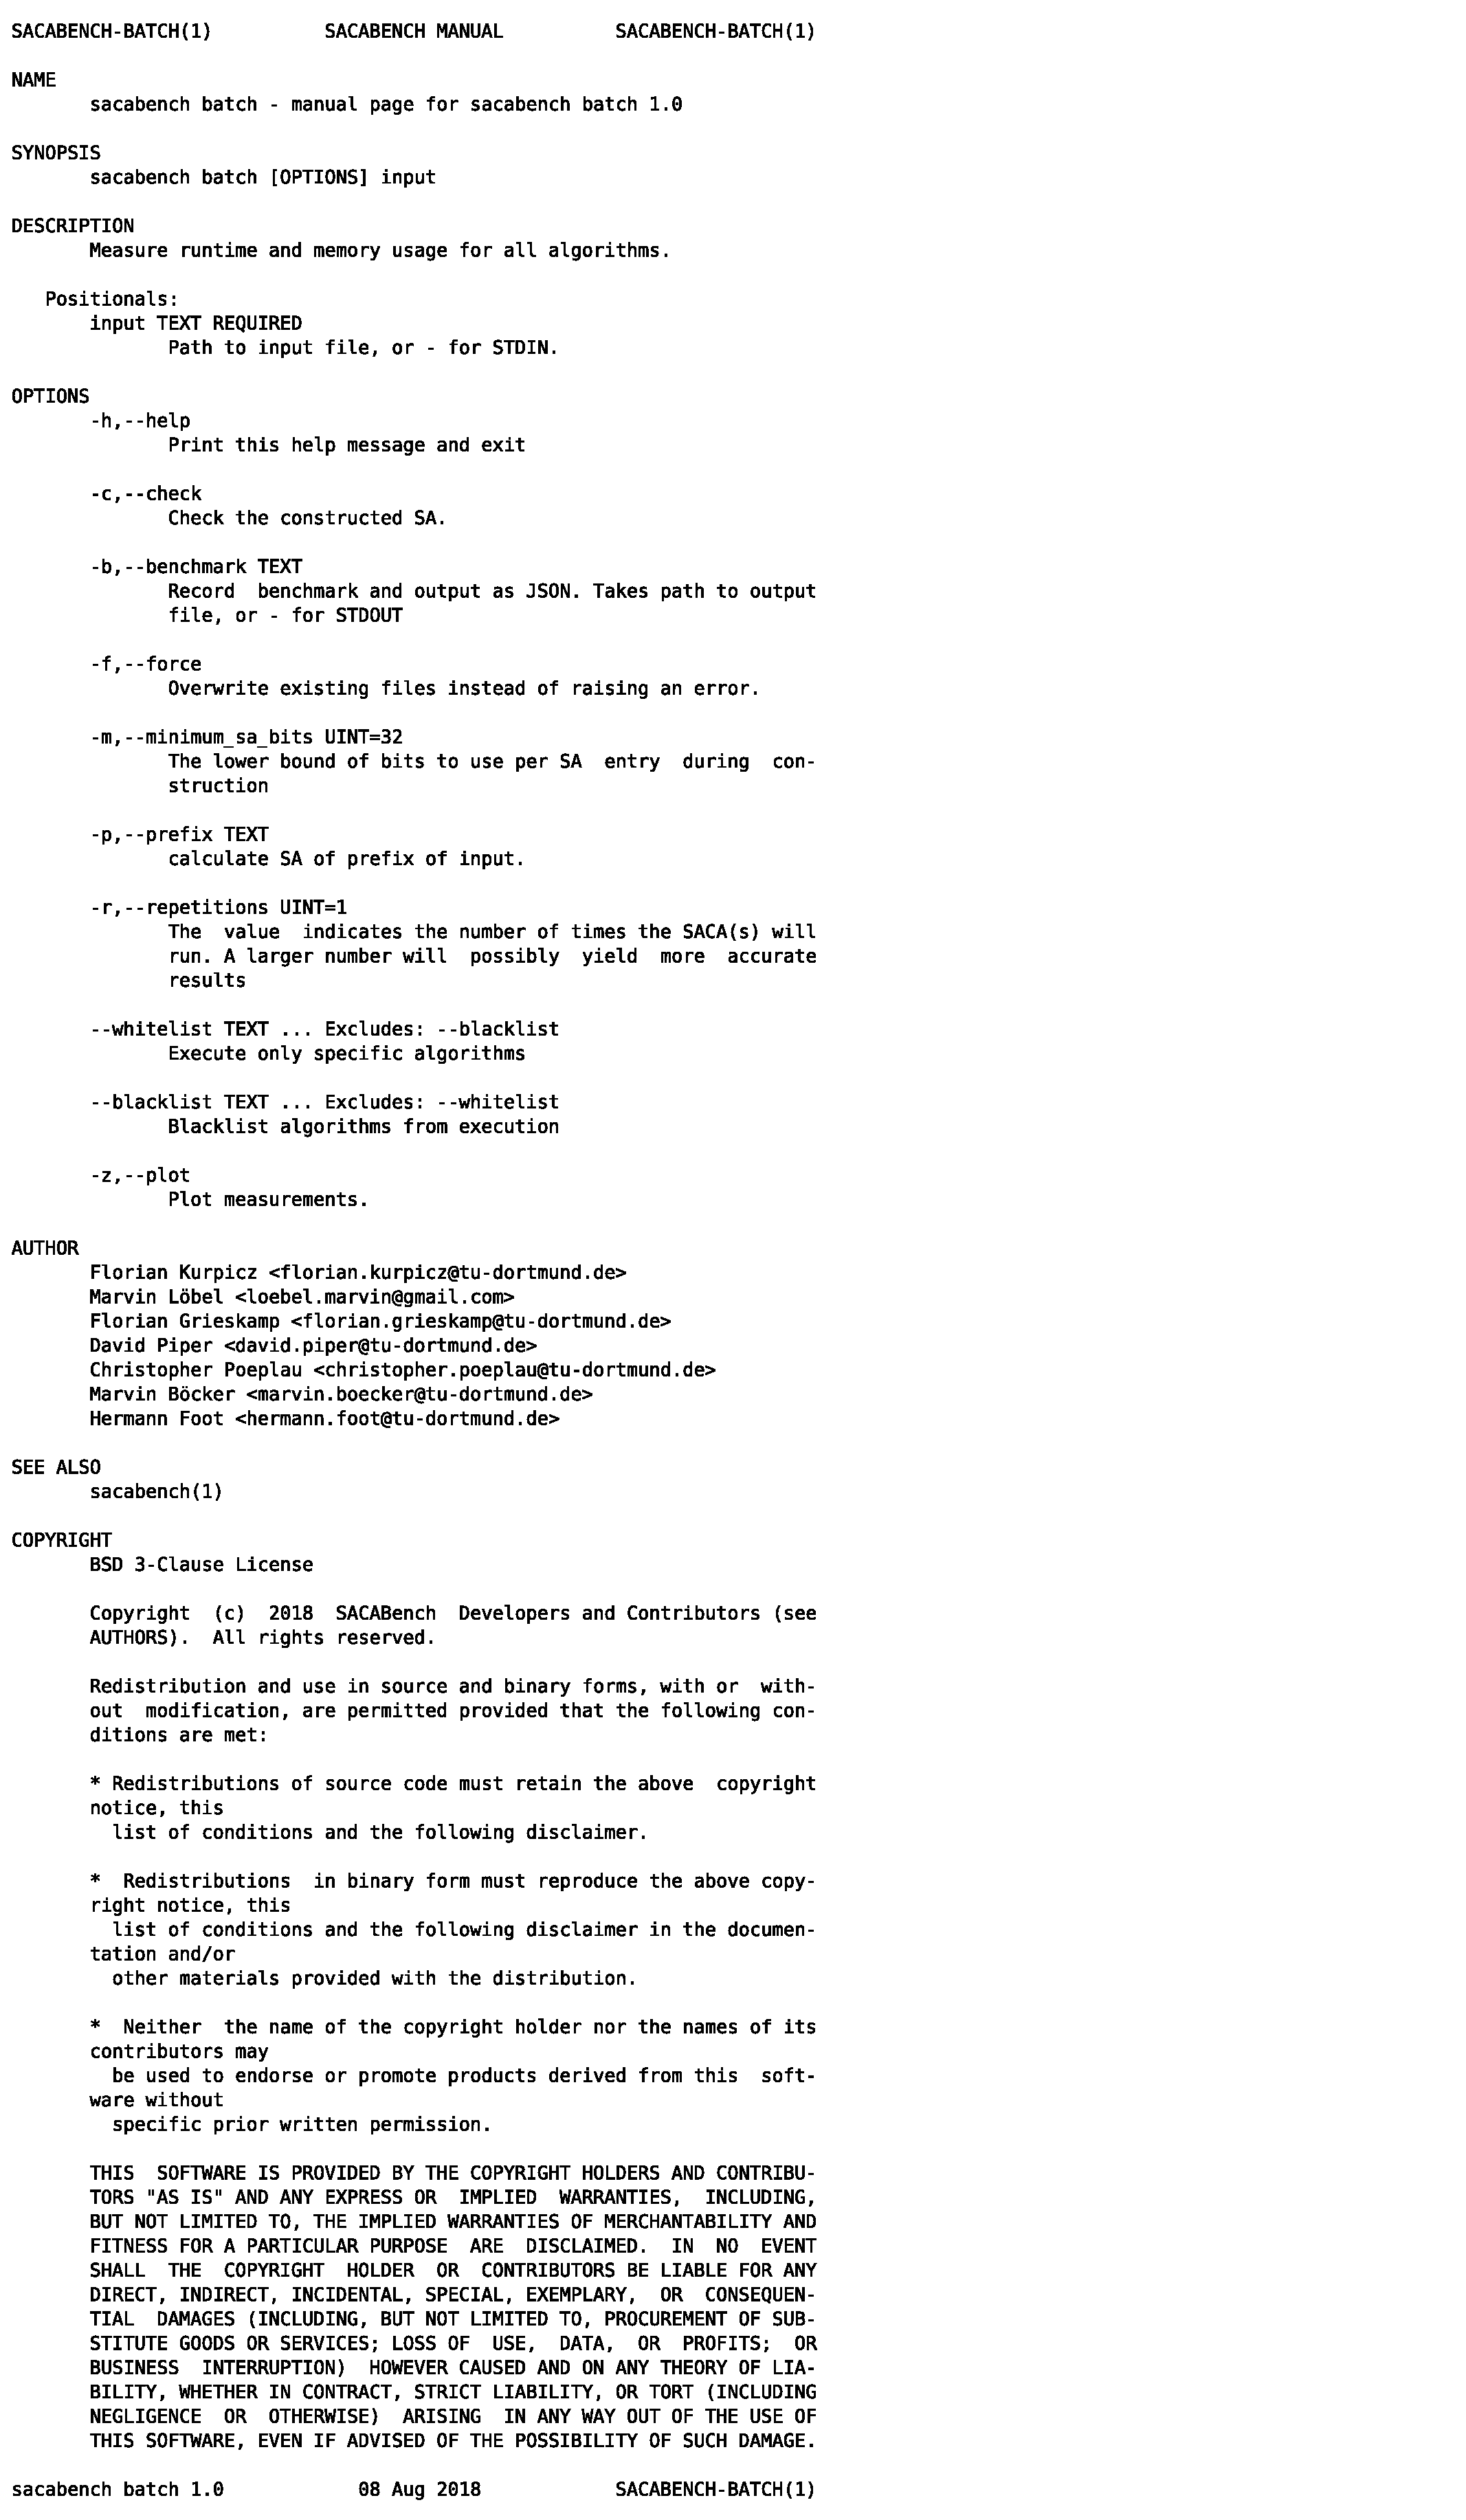
\includegraphics[page=1, viewport=0cm 25cm 20.5cm 26.3cm, clip, width=.5\textwidth]{{kapitel/3_framework/cli/sacabench-batch/sacabench-batch}.pdf}\\
    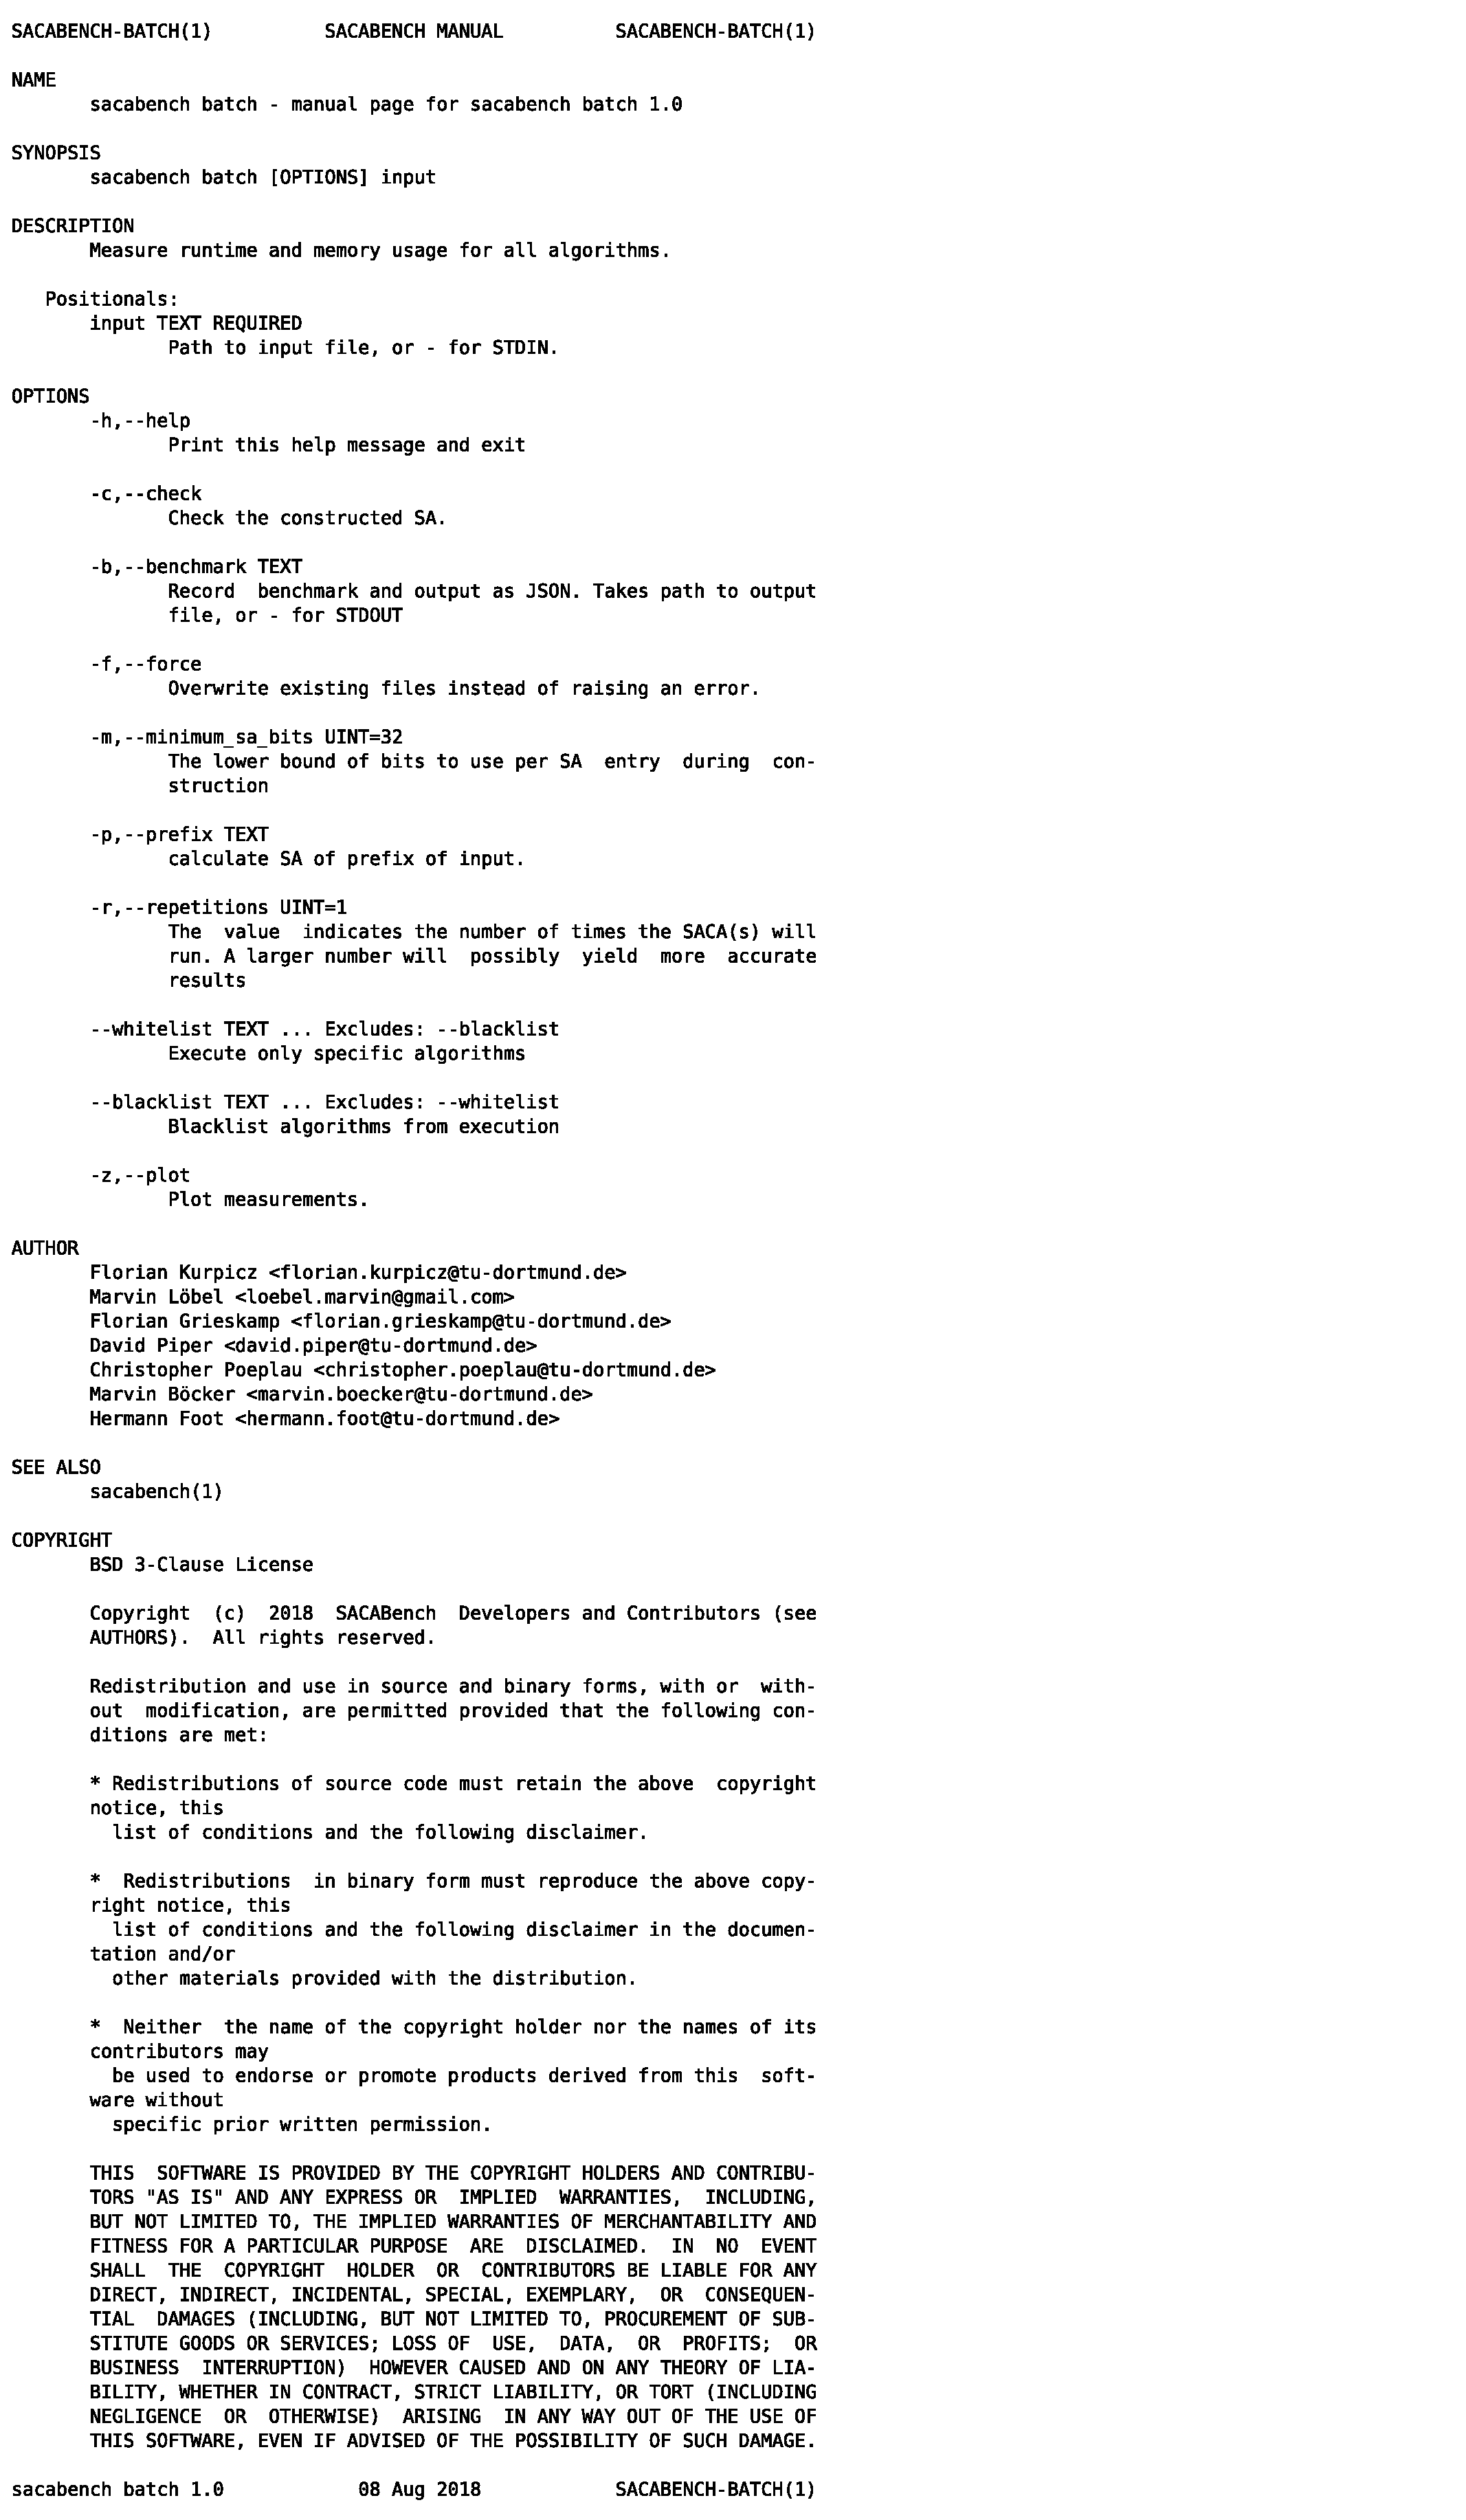
\includegraphics[page=1, viewport=0cm 0cm 20.5cm 1.5cm, clip, width=.5\textwidth]{{kapitel/3_framework/cli/sacabench-batch/sacabench-batch}.pdf}
    \caption{gekürzte Ausgabe von \texttt{man sacabench batch}}
    \label{manpage:sacabench-batch}
\end{wrapfigure}

Mit dem Befehl \texttt{sacabench batch} können mehrere Algorithmen auf der gleichen Eingabedatei ausgeführt werden. Die Funktionalität setzt hautpsächlich auf dem Interface von \termfont{sacabench construct} auf, weshalb ein Großteil der dort verwendbaren Optionen auch hier Anwendung findet. Zu Beachten ist jedoch, dass die Ausgaben aller Algorithmen nach der Ausführung und einem optionalen Test auf Korrektheit verworfen werden. Alle das Ausgabeformat betreffenden Optionen von \termfont{sacabench construct} sind daher für \termfont{sacabench batch} ungültig.\par
Um nicht für jede Messung alle Algorithmen ausführen zu müssen, besteht die Option, wahlweise mit \termfont{-{}-blacklist} einzelne Algorithmen von der Ausführung auszuschließen oder mit \termfont{-{}-white\-list} nur explizit angegebene Algorithmen zu berechnen. Für beide Optionen entsprechen die Namen der anzugebenden Algorithmen denen aus \termfont{sacabench list} (\cref{framework:cli:sacabench-list}).
Benchmarks können wie genau wie zuvor mit \termfont{-{}-benchmark} unter Angabe eines Dateinamens angelegt werden. Die mit \termfont{-{}-plot} generierten Diagramme unterscheiden sich jedoch von den mit \termfont{sacabench construct} erstellten Diagrammen: Der Schwerpunkt liegt hier auf der Vergleichbarkeit der Algorithmen, weshalb in den Diagrammen gezielt die Laufzeit- und Speichermessungen aller ausgeführten Algorithmen miteinander verglichen werden. Eine ausführlichere Beschreibung der Diagramme sowie der zur Aufzeichnung der Benchmakrs verwendeten Techniken ist in \cref{framework:benchmarks} zu finden.\par
}

